%%%%%%%%%%%%
%
% $Autor:  $
% $Datum: 11.06.2024 $
% $Pfad: DemonstratorSchrittmotor\Assembly\Chapters\de\VorMontage.tex $
% $Version: 1 $
% !TeX spellcheck = en_GB/de_DE
% !TeX encoding = utf8
% !TeX root = MontageDemontageanleitung 
% !TeX TXS-program:bibliography = txs:///biber
%%%%%%%%%%%%



\chapter{Gehäuse}

\section{Fertigung}

Die Gehäuseteile werden mithilfe einer CAD-Software konstruiert und als STL-Dateien exportiert. Anschließend erfolgt die Aufbereitung der Daten mit einer Slicer-Software, um sie an den jeweiligen 3D-Drucker anzupassen. Nach der Slicer-Bearbeitung können die G-Codes erzeugt und an den 3D-Drucker übertragen werden, woraufhin der Druckprozess gestartet werden kann.Die STL-Dateien sind unter dem Pfad: \emph{DemonstratorSchrittmotor \textbackslash MontageAnleitung \textbackslash 3D-Print \textbackslash STL} zu finden. Wenn Sie den Original Prusa i3 MK3S+ Drucker verwenden, finden Sie die fertigen G-Codes unter dem Pfad: \emph{DemonstratorSchrittmotor \textbackslash MontageAnleitung \textbackslash 3D-Print \textbackslash GCode}. Falls Veränderungen an den original CAD Dateien erfolgen sollen, finden Sie diese für das Programm Fusion unter dem Pfad: \emph{DemonstratorSchrittmotor \textbackslash MontageAnleitung \textbackslash 3D-Print \textbackslash CAD}.

\section{Teile}

\begin{figure}[H]

	\centering
	\begin{tikzpicture}[scale=1.4]
		\tikzstyle{every node}=[font=\LARGE]
		\draw [line width=1pt, short] (5.25,10.5) -- (5.5,10.5);
		\draw [line width=1pt, short] (5.5,7.5) -- (5.75,7.5);
		\draw [line width=1pt, short] (5.5,10.5) -- (5.75,7.5);
		\draw [line width=1pt, short] (5.25,10) -- (5,10);
		\draw [line width=1pt, short] (5.25,10.5) -- (5,10.5);
		\draw [line width=1pt, short] (5,10) -- (5,10.5);
		\draw [line width=1pt, short] (5,10.5) -- (5.5,10.75);
		\draw [line width=1pt, short] (5.5,10.75) -- (5.75,10.75);
		\draw [line width=1pt, short] (7.25,11.75) -- (7.75,12);
		\draw [line width=1pt, short] (5.25,7.5) -- (5.5,7.5);
		\draw [line width=1pt, short] (5.25,7.75) -- (5.25,7.5);
		\draw [line width=1pt, short] (5.25,7.75) -- (5.5,7.75);
		\draw [line width=1pt, short] (5.25,7.75) -- (5.5,8);
		\draw [line width=1pt, short] (5.5,7.75) -- (5.25,10);
		\draw [line width=1pt, short] (5.75,7.5) -- (8.5,9.25);
		\draw [line width=1pt, short] (8.5,9.25) -- (8.25,12);
		\draw [line width=1pt, short] (5.5,10.5) -- (8.25,12);
		\draw [line width=1pt, short] (7.75,12) -- (8.25,12);
		\draw [line width=1pt, short] (5.75,10.75) -- (7.5,11.75);
		\draw [line width=1pt, short] (7.25,11.75) -- (7.5,11.75);
		
	\end{tikzpicture}
	
	\caption{Platte groß}
	\label{tikz:Pg}
\end{figure}

\raggedright


\begin{figure}[H]

	\centering
	\begin{tikzpicture}[scale=0.6]
		\tikzstyle{every node}=[font=\LARGE]
		\draw [line width=1pt, short] (10,5.25) -- (10.25,-2);
		\draw [line width=1pt, short] (10,5.25) -- (15,7.75);
		\draw [line width=1pt, short] (10.25,-2) -- (15.25,1);
		\draw [line width=1pt, short] (15.25,1) -- (15,7.75);
		\draw [line width=1pt, short] (10,5.25) -- (9.25,5.5);
		\draw [line width=1pt, short] (15,7.75) -- (14.25,8);
		\draw [line width=1pt, short] (10.25,-2) -- (9.5,-1.5);
		\draw [line width=1pt, short] (9.5,-0.75) -- (9.5,-1.5);
		\draw [line width=1pt, short] (9.5,-0.75) -- (9.75,-1);
		\draw [line width=1pt, short] (9.5,4.75) -- (9.75,-1);
		\draw [line width=1pt, short] (9.25,5.5) -- (9.25,4.5);
		\draw [line width=1pt, short] (9.25,4.5) -- (9.5,4.75);
		\draw [line width=1pt, short] (9.25,5.5) -- (10.25,6);
		\draw [line width=1pt, short] (14.25,8) -- (13.25,7.5);
		\draw [line width=1pt, short] (13.25,7.5) -- (13.5,7.5);
		\draw [line width=1pt, short] (13.5,7.5) -- (10.5,6);
		\draw [line width=1pt, short] (10.25,6) -- (10.5,6);
		\draw [line width=1pt, short] (9.5,-0.75) -- (9.75,-0.5);
		\draw [ line width=1pt ] (12.25,3.75) ellipse (0.25cm and 0.25cm);
		\node [font=\LARGE] at (12.75,3.75) {};
		\draw [ line width=1pt ] (12.25,2) ellipse (0.25cm and 0.25cm);
		\draw [line width=1pt, short] (12.25,4) .. controls (12.5,3.75) and (12.25,3.75) .. (12.25,3.5);
		\draw [line width=1pt, short] (12.25,2.25) .. controls (12.5,2) and (12.25,2) .. (12.25,1.75);
	\end{tikzpicture}
	
	\caption{Platte klein}
	\label{tikz:Pk}
\end{figure}

\raggedright

\raggedright



\begin{figure}[H]
	\vspace{0.5cm}
	\centering
\begin{tikzpicture}[scale=0.6]
	\tikzstyle{every node}=[font=\LARGE]
	\draw [line width=1pt] (10.5,2.75) -- (20.25,5);
	\draw [line width=1pt] (5.75,10) -- (7.5,10.25);
	\draw [line width=1pt] (5.75,10) -- (9,8);
	\draw [line width=1pt] (9,8) -- (9,6.25);
	\draw [line width=1pt] (5.75,10) -- (5.75,8.25);
	\draw [line width=1pt] (10,8) -- (6.75,9.75);
	\draw [line width=1pt] (6.75,9.75) -- (8,10);
	\draw [line width=1pt] (7.5,10.25) -- (8,10);
	\draw [line width=1pt] (7.75,4.75) -- (7.75,7);
	\draw [line width=1pt] (8,9.25) -- (8,9.75);
	\draw [line width=1pt] (7.75,4.75) -- (10.5,2.75);
	\draw [line width=1pt] (10.5,2.75) -- (10.5,9);
	\draw [line width=1pt] (10.5,9) -- (20.25,10.5);
	\draw [line width=1pt] (20.25,5) -- (20.25,10.5);
	\draw [line width=1pt] (7.75,10.5) -- (7.75,9.25);
	\draw [line width=1pt] (6.5,7.75) -- (7,8.25);
	\draw [line width=1pt] (7,8.25) -- (8,7.75);
	\draw [line width=1pt] (8,7.75) -- (8,7);
	\draw [line width=1pt] (6.5,7.75) -- (5.75,8.25);
	\draw [line width=1pt] (8,7) -- (9,6.25);
	\draw [line width=1pt] (6.5,7.75) -- (7.75,7.75);
	\draw [line width=1pt] (7.75,8) -- (7.75,7);
	\draw [line width=1pt] (10.5,9) -- (7.75,10.5);
	\draw [line width=1pt] (7.75,10.5) -- (17.25,11.75);
	\draw [line width=1pt] (20.25,10.5) -- (17.25,11.75);
	\draw [line width=1pt] (9,6.25) -- (10,6);
	\draw [line width=1pt] (9,8) -- (10,7.75);
    \draw [line width=1pt] (10,7.75) -- (10,6);
    \draw [line width=1pt] (10,8) -- (10,7.75);
    \end{tikzpicture}
	
	\caption{Körper links}
	\label{tikz:Kl}
\end{figure}

\raggedright

\chapter{Vorbereitung der Elektronik}

\section{Anbringung der Lochscheibe des Geschwindigkeitssensors LM393}

Zur Messung der Geschwindigkeit wird die Lochscheibe des Sensors an der Stirnfläche der freiliegenden Spindel befestigt. Dies geschieht über die genaue Ausrichtung des Zylinderschraubenkopfes und einer Lötverbindung zwischen dieser und der Spindel. Eine mittige und horizontale Ausrichtung ist hierbei gefordert. Zur Kontrolle der Befestigung kann die Spindel händisch gedreht werden. Bei einem unrunden Drehlauf, kann das Lötmaterial erhitzt und eine erneute Ausrichtung durchgeführt werden. Treten nach mehreren Korrekturversuchen Haftungsprobleme auf, wird eine gründliche Entfettung und Aufrauung der Kontaktflächen empfohlen.


\begin{figure}[H]
	\vspace{0.5cm}
	\centering
	\begin{tikzpicture}[
		scale=0.2,
		every node/.style={font=\fontsize{8pt}{10pt}\selectfont\bfseries}
		]
		\draw [ line width=1pt ] (14.5,10) rectangle (16.75,-16.75);
		\draw [ line width=1pt , dashed] (14.5,2) rectangle  (16.75,0.75);
		\draw [ line width=1pt ] (14.5,2) rectangle (4,0.75);
		\draw [ line width=1pt ] (16.75,2) rectangle (17.5,0.75);
		\draw [ line width=1pt ] (17.5,1.75) rectangle (19.5,1);
		\draw [line width=1pt] (9,0.75) -- (10,-12);
		\draw [line width=1pt] (16.75,-8.25) -- (17,-11.75);
		\draw [line width=1pt] (18.5,1) -- (20.25,-11.75);
		\draw [line width=1pt] (16.75,0.75) -- (18.5,-11.75);
		
		% Knoten mit angepasster Schrift
		\node at (10,-12.5) {1};
		\node at (17,-12.5) {2};
		\node at (18.5,-12.5) {3};
		\node at (20.25,-12.5) {4};
		
	\end{tikzpicture}
	
	1 - Spindel; 2 - Frästischseite rechts; 3 - Lötzinn; 4 - Zylinderkopfschraube M5; 
	
	\caption{Achsausrichtung der Lochscheibe}
	\label{tikz:LScheibe}
\end{figure}

\raggedright


\begin{figure}[H]
	\vspace{1.5cm}
	\centering
	\tikzset{short/.style={}}
	\begin{tikzpicture}[scale=0.2, xscale=-1,
		every node/.style={font=\fontsize{800pt}{1000pt}\selectfont\bfseries}] 
		\tikzstyle
		\draw [ line width=1pt ] (31.5,-0.75) ellipse (4.5cm and 9cm);
		\draw [ line width=1pt , rotate around={90:(31.5,-0.75)}] (31.5,-0.75) ellipse (1.5cm and 1cm);
		\draw [ line width=1pt , rotate around={90:(39.5,-0.5)}] (39.5,-0.5) ellipse (1.5cm and 1cm);
		\draw [ fill={rgb,255:red,253; green,253; blue,253} , line width=1pt ] (51.25,-0.75) ellipse (2.25cm and 3.25cm);
		\draw [ line width=1pt , rotate around={90:(51.25,-0.75)}] (51.25,-0.75) ellipse (1.5cm and 1cm);
		\draw [line width=1pt, short] (48.5,2.75) -- (51.25,2.5);
		\draw [line width=1pt, short] (48,-3.75) -- (51,-4);
		\draw [line width=1pt, short] (43.25,1) -- (46.5,1);
		\draw [line width=1pt, short] (43,-2) -- (46.5,-2.25);
		\draw [line width=1pt, short] (43,-2) .. controls (42.25,-1.25) and (42.25,0.5) .. (43.25,1);
		\draw [line width=1pt, short] (29.75,8.5) -- (31.75,8.25);
		\draw [line width=1pt, short] (29.75,-9.5) -- (31.25,-9.75);
		\draw [line width=1pt, short] (48.5,2.75) .. controls (46.25,2.75) and (45,-2) .. (48,-3.75);
		\draw [line width=1pt, short] (29.75,8.5) .. controls (23.75,6) and (25,-8.25) .. (29.75,-9.5);
		\draw [ line width=1pt ] (31.5,-0.75) ellipse (2cm and 3.75cm);
		\draw [ line width=1pt ] (31.5,-0.75) ellipse (4cm and 8.5cm);
		\draw [line width=1pt, short] (31.5,7.75) -- (31.5,3);
		\draw [line width=1pt, short] (31.25,7.75) -- (31.25,3);
		\draw [line width=1pt, short] (31.5,-4.5) -- (31.5,-9.25);
		\node [font=\LARGE] at (32,5) {};
		\node [font=\LARGE] at (32.25,4.5) {};
		\draw [line width=1pt, short] (31.25,-4.5) -- (31.25,-9.25);
		\draw [line width=1pt, short] (31,0.5) .. controls (32,-0.25) and (31.5,-1.5) .. (31,-2);
		\draw [line width=1pt, short] (33.5,6.5) -- (32.5,2.5);
		\draw [line width=1pt, short] (33.75,6.25) -- (32.75,2.25);
		\node [font=\LARGE] at (33.5,4) {};
		\draw [line width=1pt, short] (30.5,-4) -- (29.5,-8);
		\draw [line width=1pt, short] (30.75,-4.25) -- (29.75,-8.25);
		\draw [line width=1pt, short] (32.25,-4.25) -- (33.75,-7.75);
		\draw [line width=1pt, short] (29.25,6.25) -- (30.5,2.5);
		\draw [line width=1pt, short] (32.5,-4) -- (34,-7.5);
		\draw [line width=1pt, short] (29,6) -- (30.25,2.25);
		\draw [line width=1pt, short] (28,3) -- (29.75,1.25);
		\draw [line width=1pt, short] (27.75,2.5) -- (29.75,0.75);
		\draw [line width=1pt, short] (33.25,-3) -- (35.25,-4.25);
		\draw [line width=1pt, short] (33.25,-2.5) -- (35.25,-3.75);
		\draw [line width=1pt, short] (33.25,1.5) -- (35,3);
		\draw [line width=1pt, short] (33.25,1) -- (35.25,2.75);
		\draw [line width=1pt, short] (33.5,-0.25) -- (35.5,0);
		\draw [line width=1pt, short] (33.5,-0.75) -- (35.5,-0.5);
		\draw [line width=1pt, short] (27.5,-1) .. controls (28.25,-0.75) and (28.5,-0.75) .. (29.5,-0.75);
		\draw [line width=1pt, short] (27.5,-1.5) .. controls (28.25,-1.25) and (28.5,-1.25) .. (29.5,-1.25);
		\draw [line width=1pt, short] (28,-5) -- (29.75,-2.75);
		\draw [line width=1pt, short] (28.25,-5.5) -- (30,-3);
		\draw [ line width=1pt , rotate around={90:(23.5,-0.75)}] (23.5,-0.75) ellipse (1.5cm and 1cm);
		\draw [ line width=1pt ] (39.5,-0.5) ellipse (2.5cm and 4.5cm);
		\draw [line width=1pt, short] (38.5,4) .. controls (35.25,2.75) and (36.25,-4.75) .. (38.75,-5);
		\draw [line width=1pt, short] (39.5,4) -- (38.5,4);
		\draw [line width=1pt, short] (39.5,-5) -- (38.75,-5);
		\draw [line width=1pt, short] (39.5,1) .. controls (40.5,0.25) and (40.5,-1.25) .. (39.5,-2);
		\draw [line width=1pt, short] (23,0.5) .. controls (23.75,0.25) and (23.75,-1.25) .. (23,-2);
		\draw [line width=1pt, short] (22.25,2) -- (21.25,0);
		\draw [line width=1pt, short] (21.25,0) -- (21.5,-2.25);
		\draw [line width=1pt, short] (22.25,2) -- (24.5,2);
		\draw [line width=1pt, short] (24.5,2) -- (25.5,0.5);
		\draw [line width=1pt, short] (25.5,0.5) -- (25.5,-2);
		\draw [line width=1pt, short] (25.5,-2) -- (24.5,-3.5);
		\draw [line width=1pt, short] (21.5,-2.25) -- (22.5,-3.5);
		\draw [line width=1pt, short] (22.5,-3.5) -- (24.5,-3.5);
		\draw [line width=1pt, short] (24.5,2) -- (22.25,2.25);
		\draw [line width=1pt, short] (24.5,-3.5) -- (21.25,-3.75);
		\draw [line width=1pt, short] (21.25,0) -- (19.5,0);
		\draw [line width=1pt, short] (21.5,-2.25) -- (19.75,-2.25);
		\draw [line width=1pt, short] (19.5,0) -- (19.75,-2.25);
		\draw [line width=1pt, short] (19.75,-2.25) -- (21.25,-3.75);
		\draw [line width=1pt, short] (22.25,2) -- (20.75,2);
		\draw [line width=1pt, short] (19.5,0) -- (20.75,2);
		\draw [line width=1pt, short] (21.25,-3.75) -- (22.5,-3.5);
		\draw [line width=1pt, short] (20.75,2) -- (22.25,2.25);
		\draw [line width=1pt, short] (30.5,-9.5) -- (29,-14.25);
		\draw [line width=1pt, short] (39.25,-5) -- (36.5,-13.75);
		\draw [line width=1pt, short] (49,-3.75) -- (45,-14);
		\draw [line width=1pt, short] (22.5,-3.75) -- (19.5,-14);
		\node [xscale=-1, transform shape] at (28.75,-15.25) {3};
		\node [xscale=-1, transform shape] at (36,-15) {2};
		\node [xscale=-1, transform shape] at (44.75,-15) {1};
		\node [xscale=-1, transform shape] at (19.25,-15) {4};
	\end{tikzpicture}
	\vspace{1cm}
	
	1 - Zylinderkopfschraube M5; 2 - Unterlegscheibe M5; 3 - Lochscheibe; 4 - Mutter M5; 
	
	\caption{Reihenfolge der Lochscheiben Anbringung}
	\label{tikz:LScheibe}
\end{figure}
\raggedright

Zur Montage der Lochscheibe wird diese zusammen mit einer Unterlegscheibe und Mutter auf der Schraube handfest angezogen. Dies ist in der Abbildung 4.2 dargestellt.



\section{Vorbereitung der elektrischen Leitungen}

Die elektrischen Leitungen werden im Vorfeld vorbereitet, um einen reibungslosen Montageprozess zu gewährleisten. Die benötigten Kabel sowie deren Anschlussarten, Längen und Bezeichnungen sind in Tabelle \ref{Leittab} aufgeführt. Bitte bereiten Sie die Kabel entsprechend für die folgenden Arbeitsschritte vor, indem Sie alle Leitungen mit der ersten Anschlusskomponente verbinden. Dies erfolgt bei über den Steckmechanismus, im Fall von Female-/Male-Anschlüssen, oder durch Schnüren und Anlöten der Leitungen an Schaltern bei abisolierten Verbindungen. Zur besseren Übersicht wird empfohlen, Leitungen mit gleicher Funktion in derselben Farbe zu verwenden.



\begin{figure}[H]
	\begin{center}
		\fontsize{8}{10}\selectfont
		\begin{tabularx}{\textwidth}{|p{0.5cm}|p{1cm}|p{2.5cm}|p{1.5cm}|p{1.5cm}|X|p{1cm}|X|} 
			\hline 
			\textbf{\newline Pos.} &  \textbf{\newline Anz. pro Leitung} &  \textbf{\newline Leitungsart \newline Pol1 - Pol2} &  \textbf{\newline Anschluss- \newline komponente 1} &  \textbf{\newline Komponente 1 Pol1} & \textbf{\newline Anschluss- \newline komponente 2} &  \textbf{\newline Komponente 2 Pol2} \\ \hline
			1 & \newline 1  & \newline abisoliert - male \newline abisoliert - male & Steckerverbinder  & \newline + \newline - & Entwicklerboard & \newline 9V \newline GND \\ \hline
			2 & \newline 2  & \newline male - female \newline male - female \newline male - male & Schrittsensor & \newline VCC \newline GND \newline Out & \newline Steckbrett \newline Stekbrett \newline Arduino & \newline + \newline - \newline P9 \\ \hline
			3 & 1 & \newline abisoliert - male \newline abisoliert - male  & Taster grün & \newline + \newline - & \newline Arduino \newline Steckbrett & \newline P4 \newline -  \\ \hline
			4 & 1 & \newline abisoliert - male \newline abisoliert - male  & Taster rot & \newline + \newline - & \newline Arduino \newline Steckbrett & \newline P5 \newline -  \\ \hline
			5 & 1 & \newline abisoliert - female \newline abisoliert - male  & Powerschalter & \newline + \newline - & \newline Arduino \newline Steckbrett & \newline P8 \newline - \\ \hline
			6 & \newline 3  & \newline female - male \newline female - male \newline female - male \newline female - male \newline female - male & \newline Arduino \newline Arduino \newline Arduino \newline Steckbrett \newline Steckbrett  & \newline CLK \newline DT \newline SW \newline + \newline GND  & \newline A1 \newline A2 \newline A3 \newline + \newline - \\ \hline
			7 & \newline 3  & \newline abisoliert - male \newline abisoliert - male & Endschalter rechts & \newline NC \newline C &  \newline Arduino \newline Steckbrett & \newline P7 \newline -  \\ \hline
			8 & \newline 3  & \newline abisoliert - male \newline abisoliert - male & Endschalter links & \newline NC \newline C &  \newline Arduino \newline Steckbrett & \newline P11 \newline -  \\ \hline
			9 & \newline 1   & \newline female - male \newline female - male \newline female - male \newline female - male \newline female - male \newline female - male \newline female - male  & Display & \newline D2 \newline A0 \newline RST \newline D1 \newline D0 \newline VDD \newline VSS & \newline Arduino \newline Arduino \newline Arduino \newline Arduino \newline Arduino \newline Steckbrett \newline Steckbrett & \newline P6 \newline P12 \newline P10 \newline A4 \newline A5 \newline + \newline - \\ \hline
			10 & \newline 1  & \newline female - male \newline female - male  & Arduino & \newline 5V \newline GND & \newline Steckbrett \newline Steckbrett & \newline + \newline -  \\ \hline
			11 & \newline 1 & \newline male - male \newline male - male \newline male - female \newline male - female  & Entwicklerboard & \newline 5V \newline GND \newline 9 \newline 8  & \newline Steckbrett \newline Steckbrett \newline Arduino \newline Arduino & \newline + \newline - \newline P3 \newline P2 \\ \hline
			12 & \newline bestehen- \newline des Anschlusskabel & \newline x - female & Schrittmotor & A1,A2,B1,B2 & Entwicklerboard & \newline Anschluss- \newline buchse  \\ \hline
			
			
		\end{tabularx}
		\captionof{table}{Leitungen}	\label{Leittab}
	\end{center}
\end{figure}


\section{Schaltplan}
Um einen Überblick zu erhalten betrachten wir den Schlatplan in Abbildung \ref{Leitungen}.

\begin{figure}[H]
	\begin{center}
		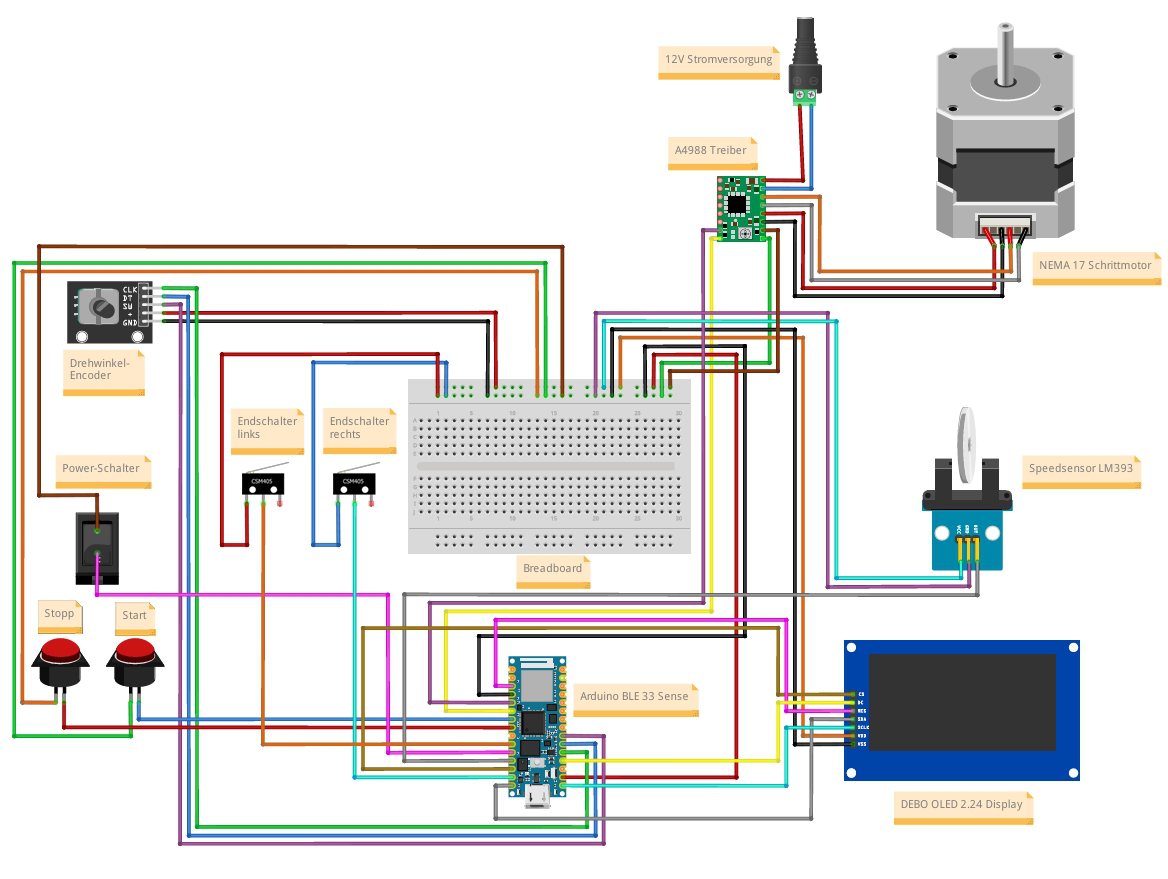
\includegraphics[width=\textwidth]{Images/Schaltplan.jpeg}
		\caption{Schaltplan} \label{Leitungen}
	\end{center}
\end{figure}




\section{Anbringung von Steckbrett und Entwicklerboard }


\begin{figure}[H]
	\vspace{1.5cm}
	\centering
	\tikzset{short/.style={}}
	\begin{tikzpicture}[scale=1, 
		every node/.style={font=\fontsize{800pt}{1000pt}\selectfont\bfseries}]
		\tikzstyle{every node}=[font=\LARGE]
		\draw [line width=1pt, short] (5.25,10.5) -- (5.5,10.5);
		\draw [line width=1pt, short] (5.5,7.5) -- (5.75,7.5);
		\draw [line width=1pt, short] (5.5,10.5) -- (5.75,7.5);
		\draw [line width=1pt, short] (5.25,10) .. controls (5.25,10.25) and (5,10) .. (5,10);
		\draw [line width=1pt, short] (5.25,10.5) -- (5,10.5);
		\draw [line width=1pt, short] (5,10) -- (5,10.5);
		\draw [line width=1pt, short] (5,10.5) -- (5.5,10.75);
		\draw [line width=1pt, short] (5.5,10.75) -- (5.75,10.75);
		\draw [line width=1pt, short] (7.25,11.75) -- (7.75,12);
		\draw [line width=1pt, short] (5.25,7.5) -- (5.5,7.5);
		\draw [line width=1pt, short] (5.25,7.75) -- (5.25,7.5);
		\draw [line width=1pt, short] (5.25,7.75) -- (5.5,7.75);
		\draw [line width=1pt, short] (5.25,7.75) -- (5.5,8);
		\draw [line width=1pt, short] (5.5,7.75) -- (5.25,10);
		\draw [line width=1pt, short] (8.5,9.25) -- (8.25,12);
		\draw [line width=1pt, short] (5.5,10.5) -- (8.25,12);
		\draw [line width=1pt, short] (7.75,12) -- (8.25,12);
		\draw [line width=1pt, short] (5.75,10.75) -- (7.5,11.75);
		\draw [line width=1pt, short] (7.25,11.75) -- (7.5,11.75);
		\draw [line width=0.6pt, short] (5.5,10.5) -- (6,10.5);
		\draw [line width=1pt, short] (5.75,7.5) -- (6.25,7.5);
		\draw [line width=1pt, short] (6.25,7.5) -- (7.5,8.25);
		\draw [line width=1pt, short] (6,10.5) -- (7.25,11.25);
		\draw [line width=1pt, short] (7.5,8.25) -- (7.25,11.25);
		\draw [line width=1pt, short] (6,10.5) -- (6.25,7.5);
		\draw [line width=1pt, short] (7.5,8.5) -- (8.5,9.25);
		\draw [line width=0.6pt, short] (6.25,10.5) -- (6.5,7.75);
		\draw [line width=0.6pt, short] (7,11) -- (7.25,8.25);
		\draw [line width=0.6pt, short] (7.25,11.25) -- (7,11.25);
	\end{tikzpicture}
	
	
	\caption{Platte groß mit Steckbrett}
	\label{tikz:Steckbrett}
\end{figure}
\raggedright


\begin{figure}[H]
	\vspace{1.5cm}
	\centering
	\tikzset{short/.style={}}
	\begin{tikzpicture}[scale=0.6, 
		every node/.style={font=\fontsize{800pt}{1000pt}\selectfont\bfseries}]
		\tikzstyle{every node}=[font=\LARGE]
		\draw [line width=1pt, short] (10,5.25) -- (15,7.75);
		\draw [line width=1pt, short] (10.25,-2) -- (15.25,1);
		\draw [line width=1pt, short] (15.25,1) -- (15,7.75);
		\draw [line width=1pt, short] (10,5.25) -- (9.25,5.5);
		\draw [line width=1pt, short] (15,7.75) -- (14.25,8);
		\draw [line width=1pt, short] (10.25,-2) -- (9.5,-1.5);
		\draw [line width=1pt, short] (9.5,-0.75) -- (9.5,-1.5);
		\draw [line width=1pt, short] (9.5,-0.75) -- (9.75,-1);
		\draw [line width=1pt, short] (9.5,4.75) -- (9.75,-1);
		\draw [line width=1pt, short] (9.25,5.5) -- (9.25,4.5);
		\draw [line width=1pt, short] (9.25,4.5) -- (9.5,4.75);
		\draw [line width=1pt, short] (9.25,5.5) -- (10.25,6);
		\draw [line width=1pt, short] (14.25,8) -- (13.25,7.5);
		\draw [line width=1pt, short] (13.25,7.5) -- (13.5,7.5);
		\draw [line width=1pt, short] (13.5,7.5) -- (10.5,6);
		\draw [line width=1pt, short] (10.25,6) -- (10.5,6);
		\draw [line width=1pt, short] (9.5,-0.75) -- (9.75,-0.5);
		\draw [ line width=1pt ] (12,4) ellipse (0.25cm and 0.25cm);
		\node [font=\LARGE] at (13.5,3.25) {};
		\draw [ line width=1pt ] (12.25,2) ellipse (0.25cm and 0.25cm);
		\draw [line width=1pt, short] (12,4.25) .. controls (12.25,4) and (12,4) .. (12,3.75);
		\draw [line width=1pt, short] (10.5,4) -- (12.5,5);
		\draw [line width=1pt, short] (12.5,5) -- (12.75,1.75);
		\draw [line width=1pt, short] (10,5.25) -- (10.25,-2);
		\draw [line width=1pt, short] (10.5,4) -- (10.75,0.5);
		\draw [line width=1pt, short] (10.75,0.5) -- (12.75,1.5);
		\draw [line width=1pt, short] (12.5,5) -- (12.75,1.5);
		\draw [ line width=1pt , rotate around={24:(11.5,2.75)}] (11.5,2) -- (11,2) -- (11.5,3.5) -- (12,3.5) -- cycle;
		\draw [line width=1pt, short] (12.25,2.25) .. controls (12.5,2) and (12.25,2) .. (12.25,1.75);
		\draw [line width=1pt, short] (10.25,4) -- (12.25,5);
		\draw [line width=1pt, short] (10.25,4) -- (10.5,0.5);
		\draw [line width=1pt, short] (10.25,4) -- (10.5,4);
		\draw [line width=1pt, short] (10.5,0.5) -- (10.75,0.5);
		\draw [line width=1pt, short] (12.25,5) -- (12.5,5);
		\draw [ line width=1pt , rotate around={36:(11,3.5)}] (10.75,3) -- (10.5,3) -- (11,3.75) -- (11.25,3.75) -- cycle;
		\draw [ line width=1pt , rotate around={36:(11,1.5)}] (10.75,1) -- (10.5,1) -- (11,1.75) -- (11.25,1.75) -- cycle;
		\node [font=\LARGE] at (13.75,2.25) {};
	\end{tikzpicture}
	
	\caption{Platte klein mit Entwicklerboard}
	\label{tikz:Steckbrett}
\end{figure}
\raggedright


	
	



\section{Schrauben und Muttern }

In der folgenden Tabelle \ref{Verbrauch} werden die benötigten Schrauben und Muttern aufgelistet

\begin{figure}[H]
	\begin{center}
		\fontsize{8}{10}\selectfont
		\begin{tabularx}{\textwidth}{|p{0.5cm}|p{0,8cm}|X|X|X|X|} 
			\hline 
			\textbf{Pos.} &  \textbf{Anzahl} &  \textbf{Beschreibung}\\ \hline
			1 & 17 & M3 Hammermutter T-Schlitz Nut 6  \\ \hline
			2 & 14 & Zylinderschrauben M3 6 \ mm Innensechskant DIN 912  \\ \hline
			3 & 16 & Zylinderschrauben M3 8 \ mm Innensechskant DIN 912 \\ \hline
			4 & 21 & Zylinderschrauben M3 10 \ mm Innensechskant DIN 912\\ \hline
			5 & 7  & Zylinderschrauben M3 14 \ mm Innensechskant DIN 912 \\ \hline
			6 & 7 & Sechskantmuttern M3 DIN 934  \\ \hline
			7 & 2 &  Senkschrauben M2.5 5 \ mm Kreuzschlitz Phillips  \\ \hline
			
		\end{tabularx}
		\captionof{table}{Benötigte Schrauben und Muttern}	\label{Verbrauch}
	\end{center}
\end{figure}

\section{Schaltplan}

Der Schaltplan zeigt die elektrische Verbindung der einzelnen Komponenten. Er ist in Abbildung \ref{Splan} dargestellt.

\begin{figure}[H]
	\begin{center}
		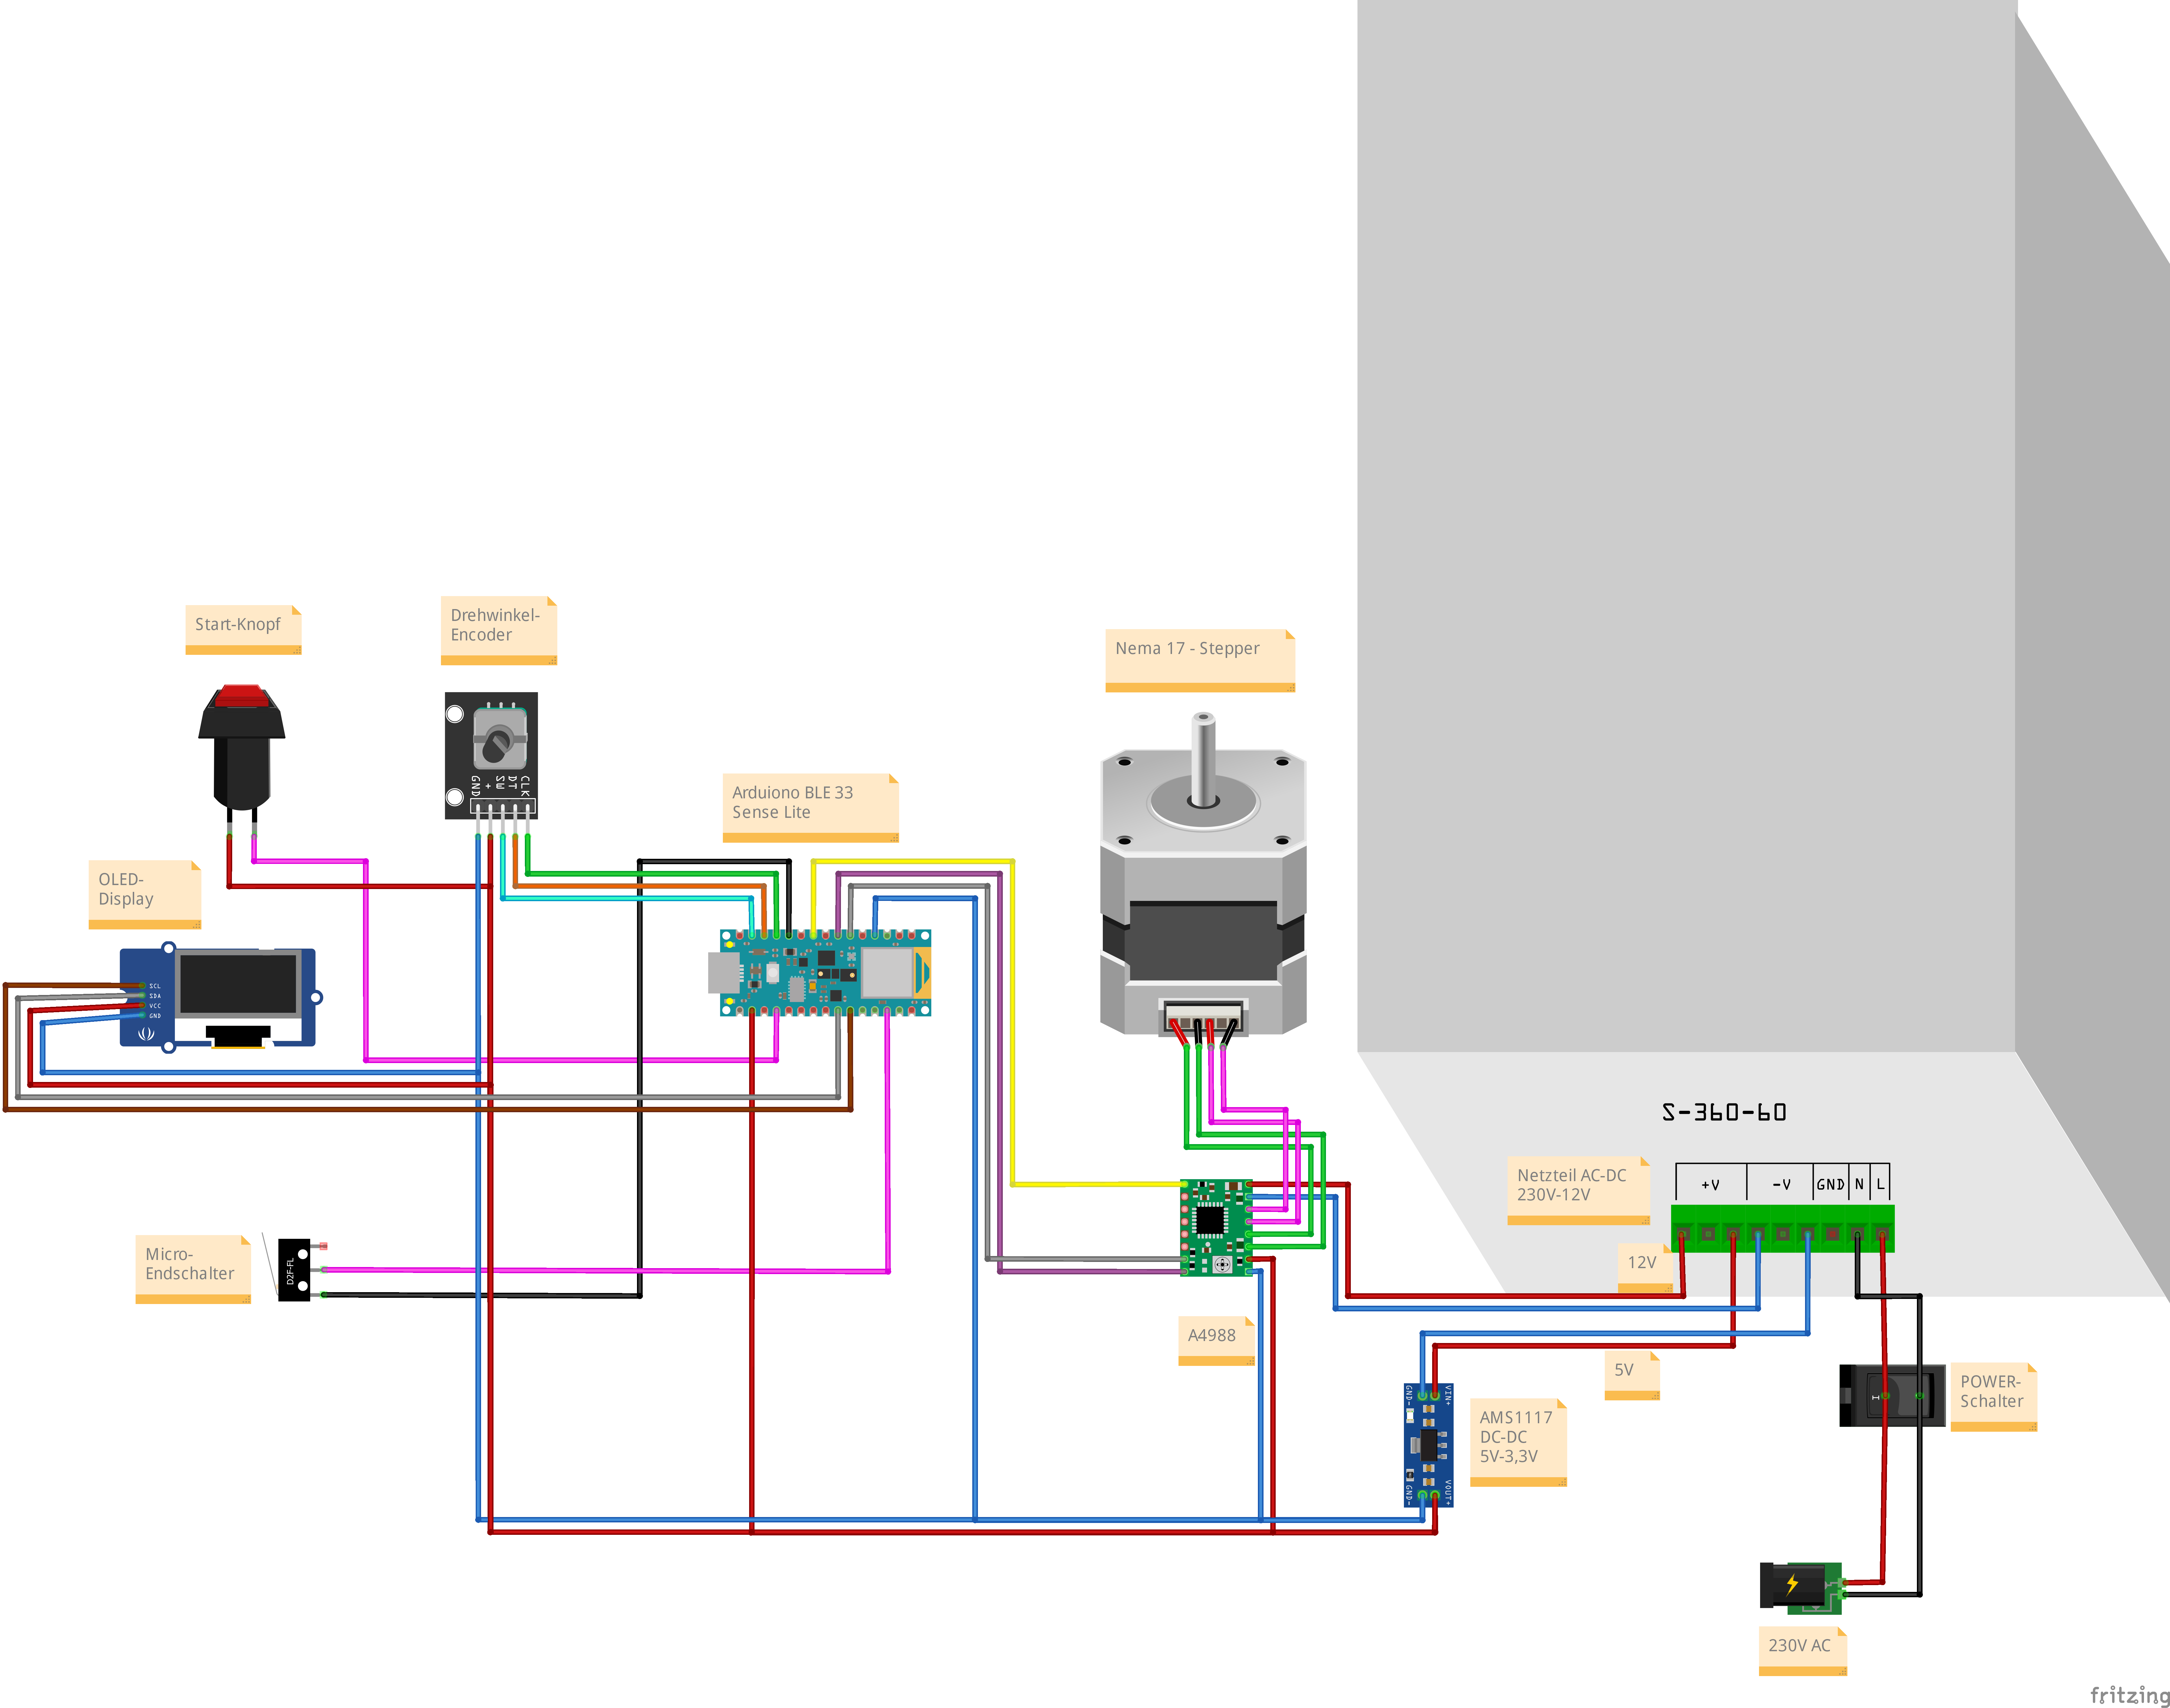
\includegraphics[width=\textwidth]{Images/Schaltplan1.png}
		\caption{Schaltplan} \label{Splan}
	\end{center}
\end{figure}



\chapter{Montage}\label{Mont}

In diesem Kapitel wird die Montage des Demonstrators für einen Schrittmotor Schritt für Schritt erläutert. Es wird empfohlen, die Schritte in der vorgegebenen Reihenfolge zu befolgen.

\section{Erster Schritt: Montieren Schaltnetzteil, Entwicklerboard und AMS1117}
 Montieren Sie die folgenden Bauteile und elektrischen Komponenten wie in Abbildung \ref{1.S} gezeigt. 
 
\begin{enumerate}
 	\item Befestigen Sie das Schaltnetzteil an der Bodenplatte mit 2 $\times$ $ M3 \times 10 \ mm $ Schrauben. Die Schrauben werden von der unteren Seite der Bodenplatte eingeführt. 
 	\item Nehmen Sie 2 $\times$ $ M3 \times 14 \ mm $ Schrauben und kontern Sie diese mit 2 $\times M3 $ Muttern gegen die Bodenplatte. Die Schrauben werden von der unteren Seite der Bodenplatte eingeführt.
 	\item Montieren Sie das Entwicklerboard Schrittmotorsteuerung A4988 auf der Bodenplatte. Verwenden Sie 2 $\times$ $ M3 \times 14 \ mm $ und 4 $\times$ $ M3 $ Muttern. Die Reihenfolge ist: Schraube - Bodenplatte - Mutter - Entwicklerboard - Mutter. Die Schrauben werden von der unteren Seite der Bodenplatte eingeführt.
 	\item Stecken Sie die Schrittmotorsteuerung in das Entwicklerboard und achten Sie auf die richtige Pinbelegung.
 	\item Setzen Sie den Spannungswandler AMS1117 in den Halter für AMS und setzen Sie den Clip auf. Befestigen Sie den Halter und den Clip mit einer  $\times$ $ M3 \times 14 \ mm $ Schraube
\end{enumerate}
 
\begin{figure}[H]
	\begin{center}
		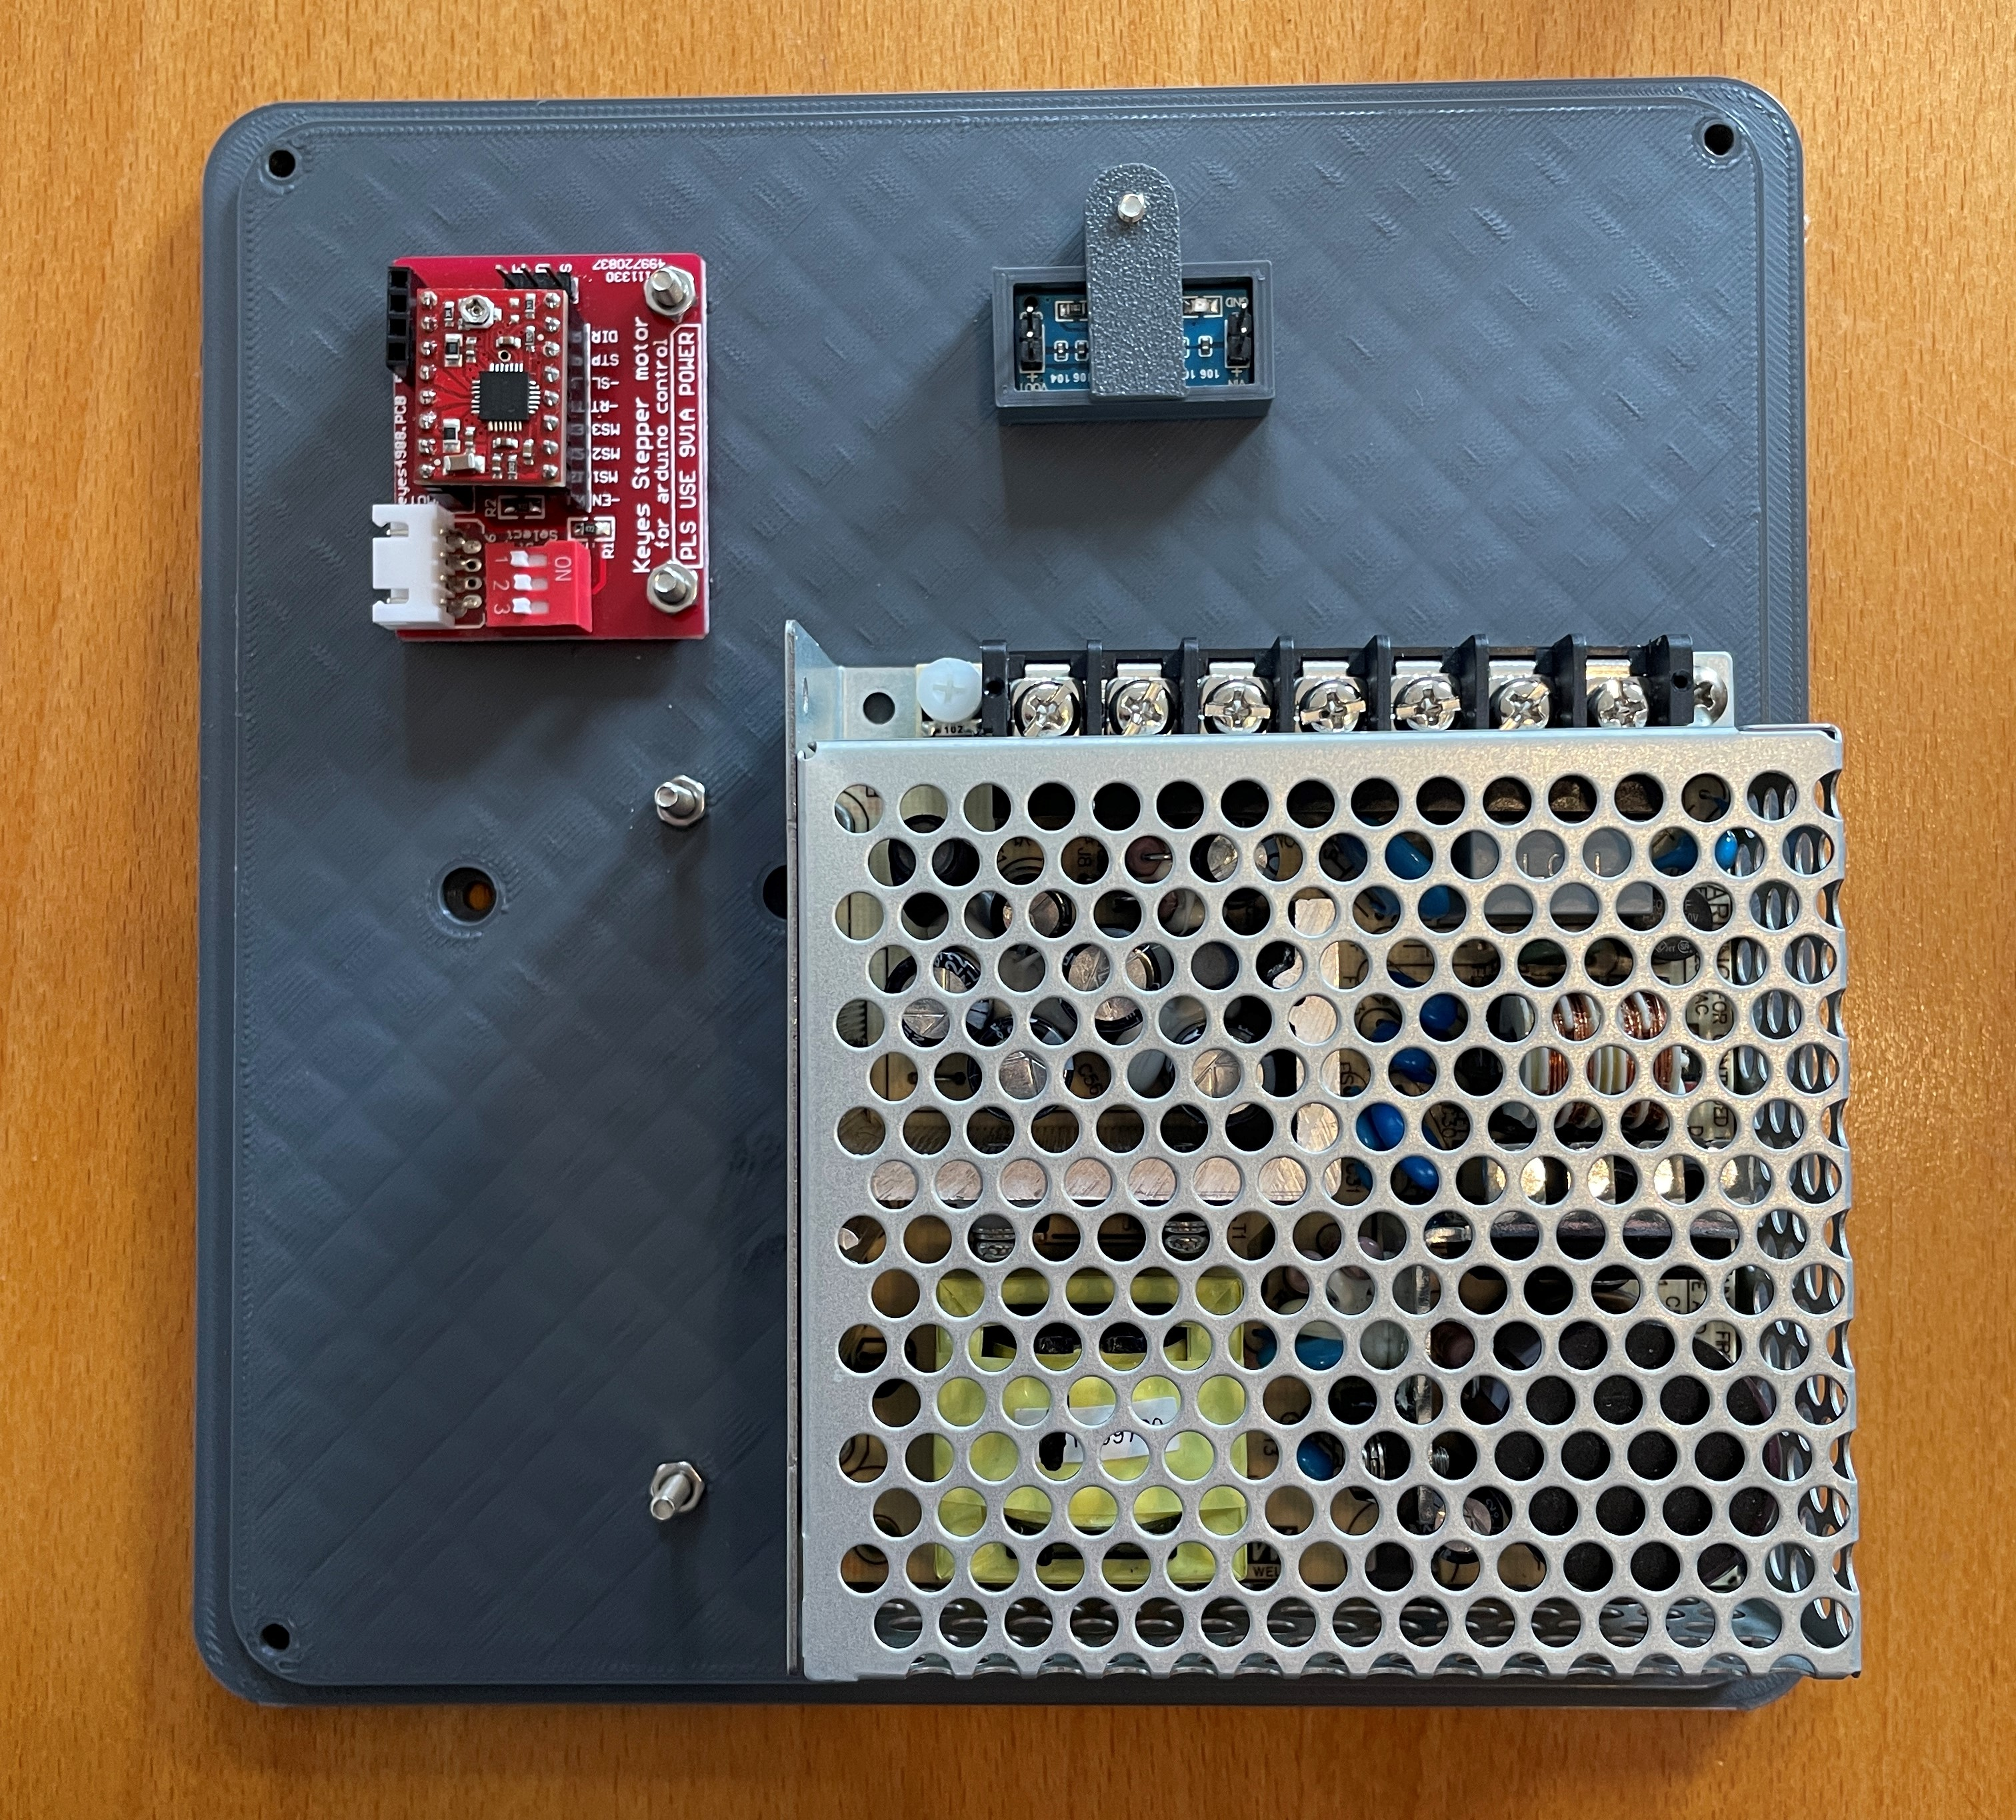
\includegraphics[width=\textwidth]{Images/1Schr.jpg}
		\caption{Erster Schritt: Montieren Schaltnetzteil, Entwicklerboard und AMS1117} \label{1.S}
	\end{center}
\end{figure}


\section{Zweiter Schritt: Anbringen der Bodenplatte an Aluprofil}

Montieren Sie die folgenden Bauteile und elektrischen Komponenten wie in Abbildung \ref{2.S} gezeigt.

\begin{enumerate}
	\item Führen Sie 2 $\times$ $ M3 $ Hammermutter in das Aluprofil ein.
	\item Verschrauben Sie die Bodenplatte mit 2 $\times$ $ M3 \times 10 \ mm $ Schrauben an den Hammermuttern im Aluprofil, sodass die Bodenplatte bündig mit dem Profil abschließt.
	\item Setzen Sie das Tiny Machine Learning Shield (TMLS) auf die hervorstehenden Schrauben und sichern Sie es mit 2 $\times$ $ M3 $ Muttern.
	Stecken Sie den Arduino Nano Sense BLE 33 Lite auf das TMLS und achten Sie dabei auf die Pinbelegung.
\end{enumerate}

\begin{figure}[H]
	\begin{center}
		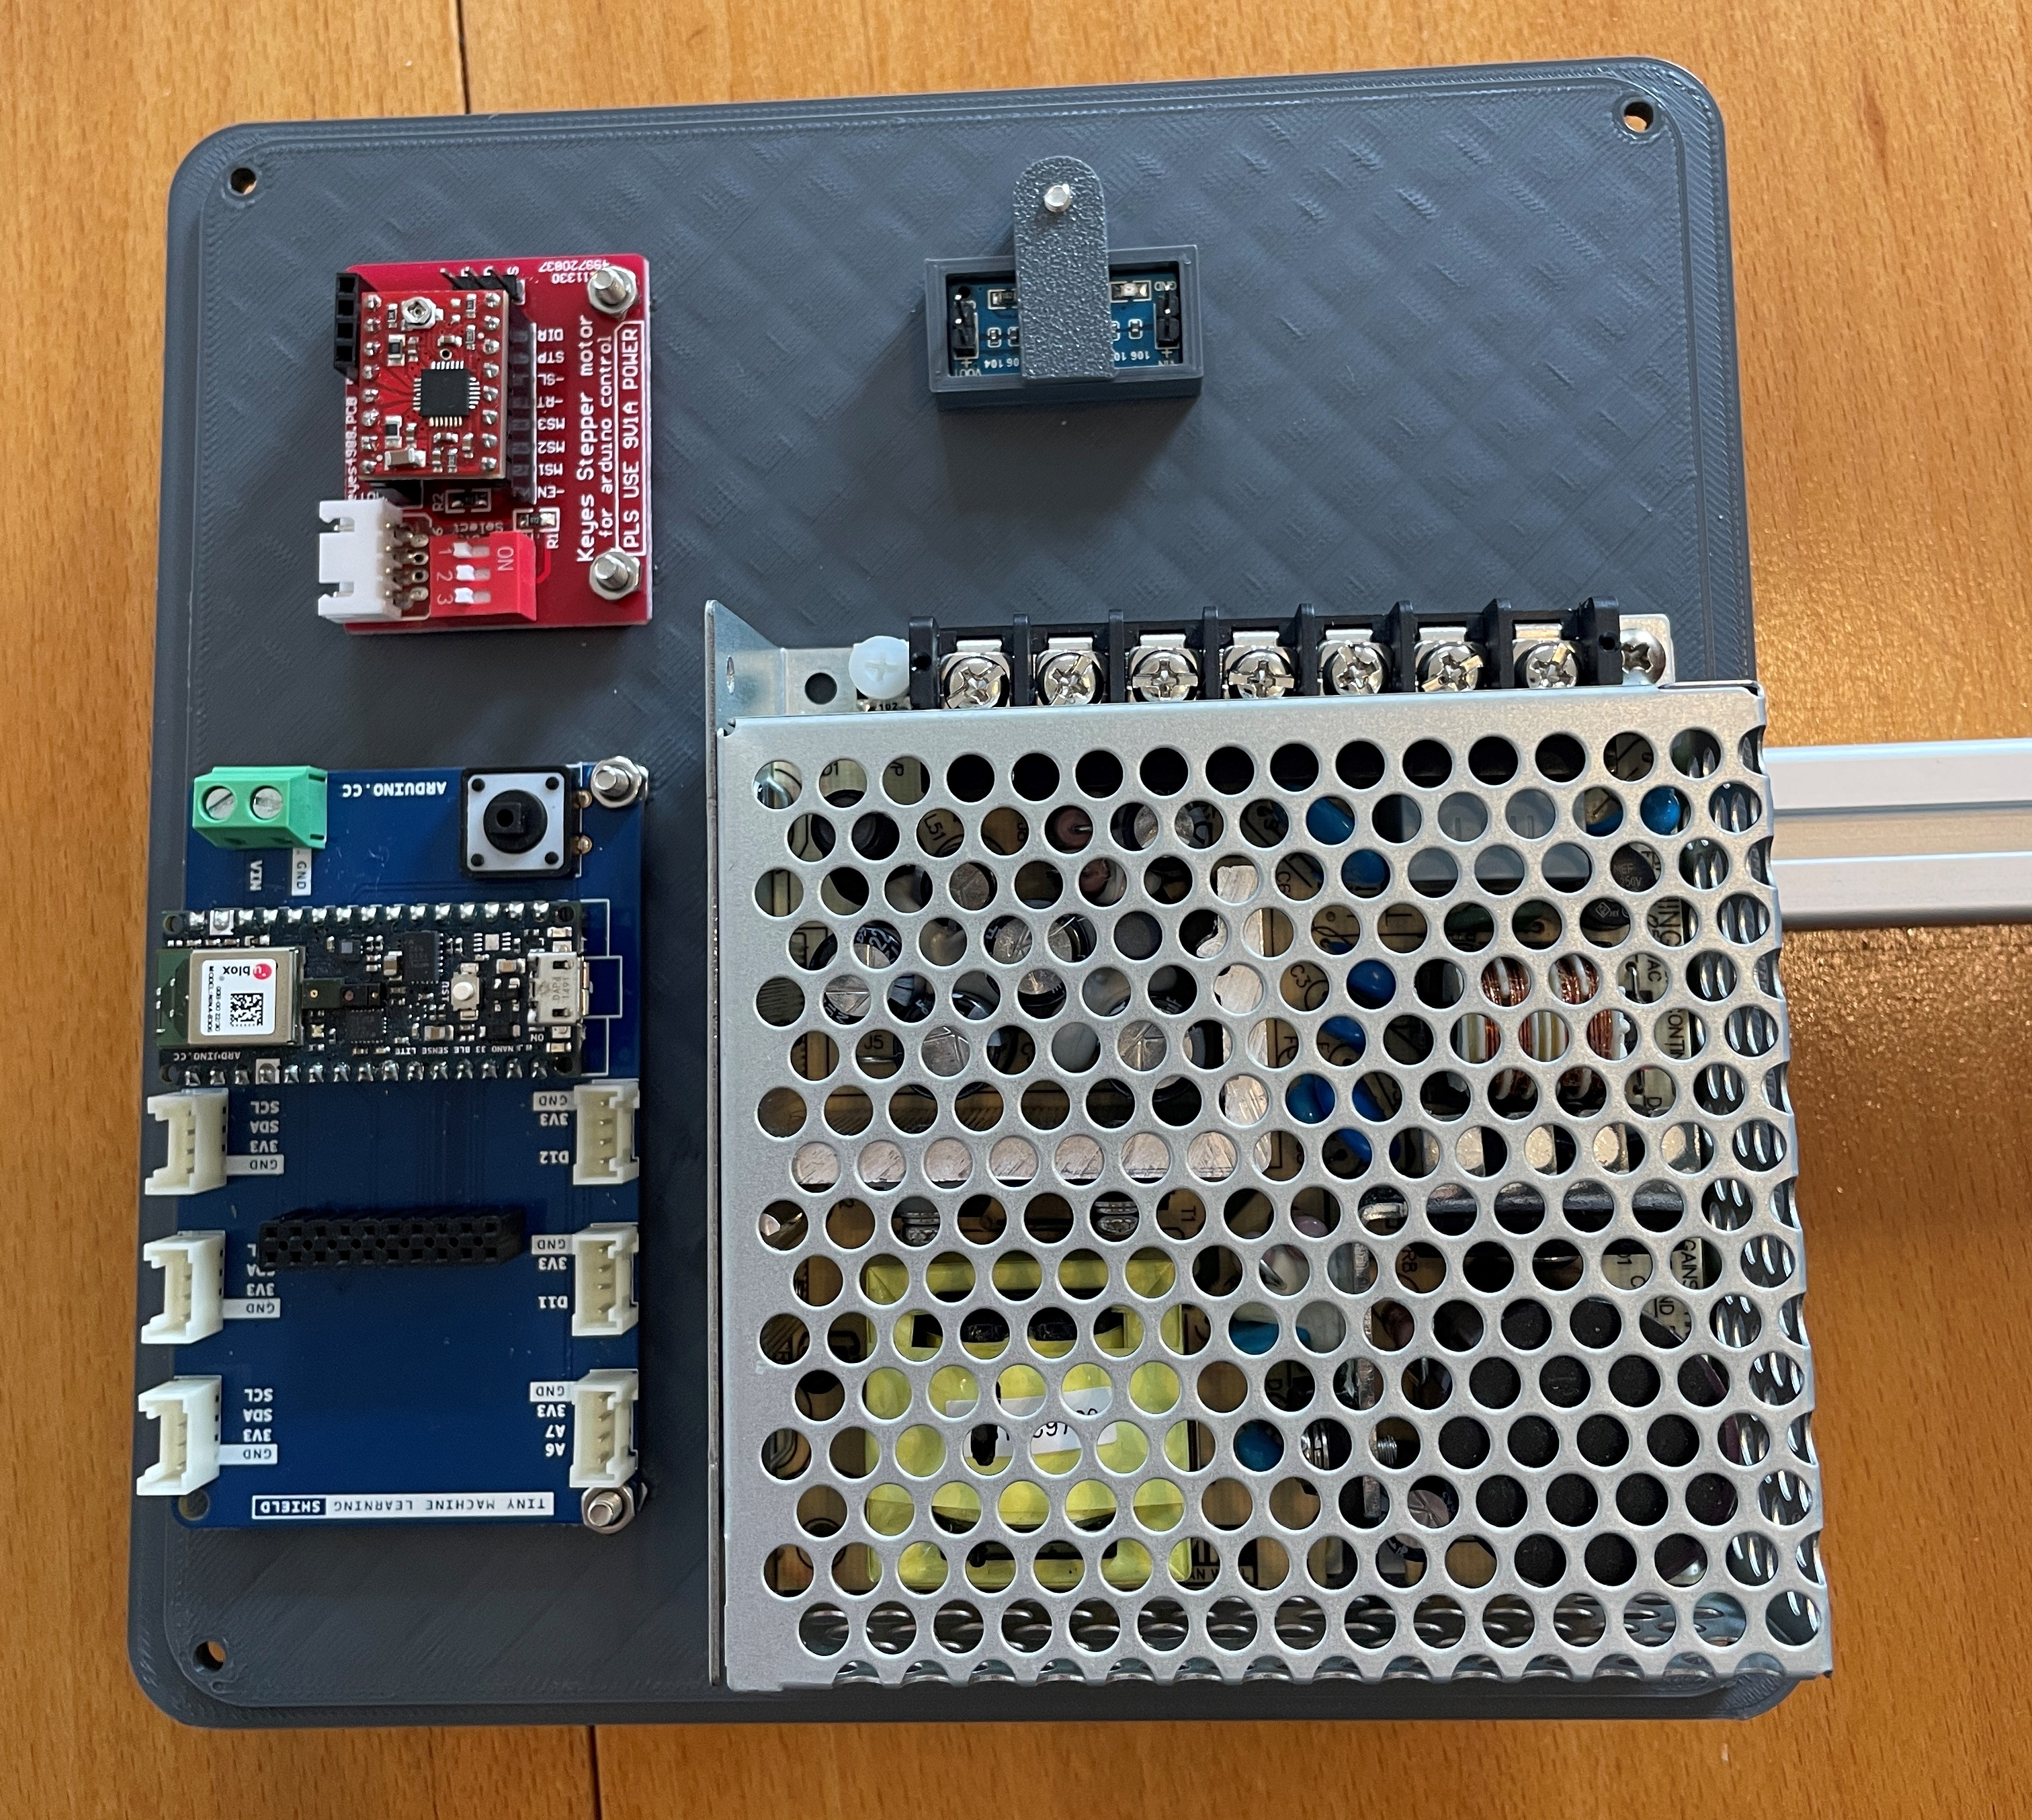
\includegraphics[width=\textwidth]{Images/2Schr.jpg}
		\caption{Zweiter Schritt: Anbringen der Bodenplatte an Aluprofil} \label{2.S}
	\end{center}
\end{figure}


\section{Dritter Schritt: Zusammenbau der Vorderplatte}

Montieren Sie die folgenden Bauteile und elektrischen Komponenten wie in Abbildung \ref{3.S} gezeigt.

\begin{enumerate}
	\item Befestigen Sie das OLED-Display mit 2 $\times$ $ M3 \times 6 \ mm $ Schrauben in die dafür vorgesehenen \O 2,8 \ mm Bohrungen der Vorderplatte.
	\item Führen Sie die SMD-LED in die \O 8 \ mm Bohrung der Vorderen Platte ein.
	\item Führen Sie den Drehwinkel-Encoder in die \O 7 \ mm Bohrung ein und kontern Sie diese mit der P-4 Mutter.
	\item Führen Sie den Druckknopf in die \O 13,5 \ mm Bohrung und kontern Sie den mit der zugehörigen Mutter.
\end{enumerate}

\begin{figure}[H]
	\begin{center}
		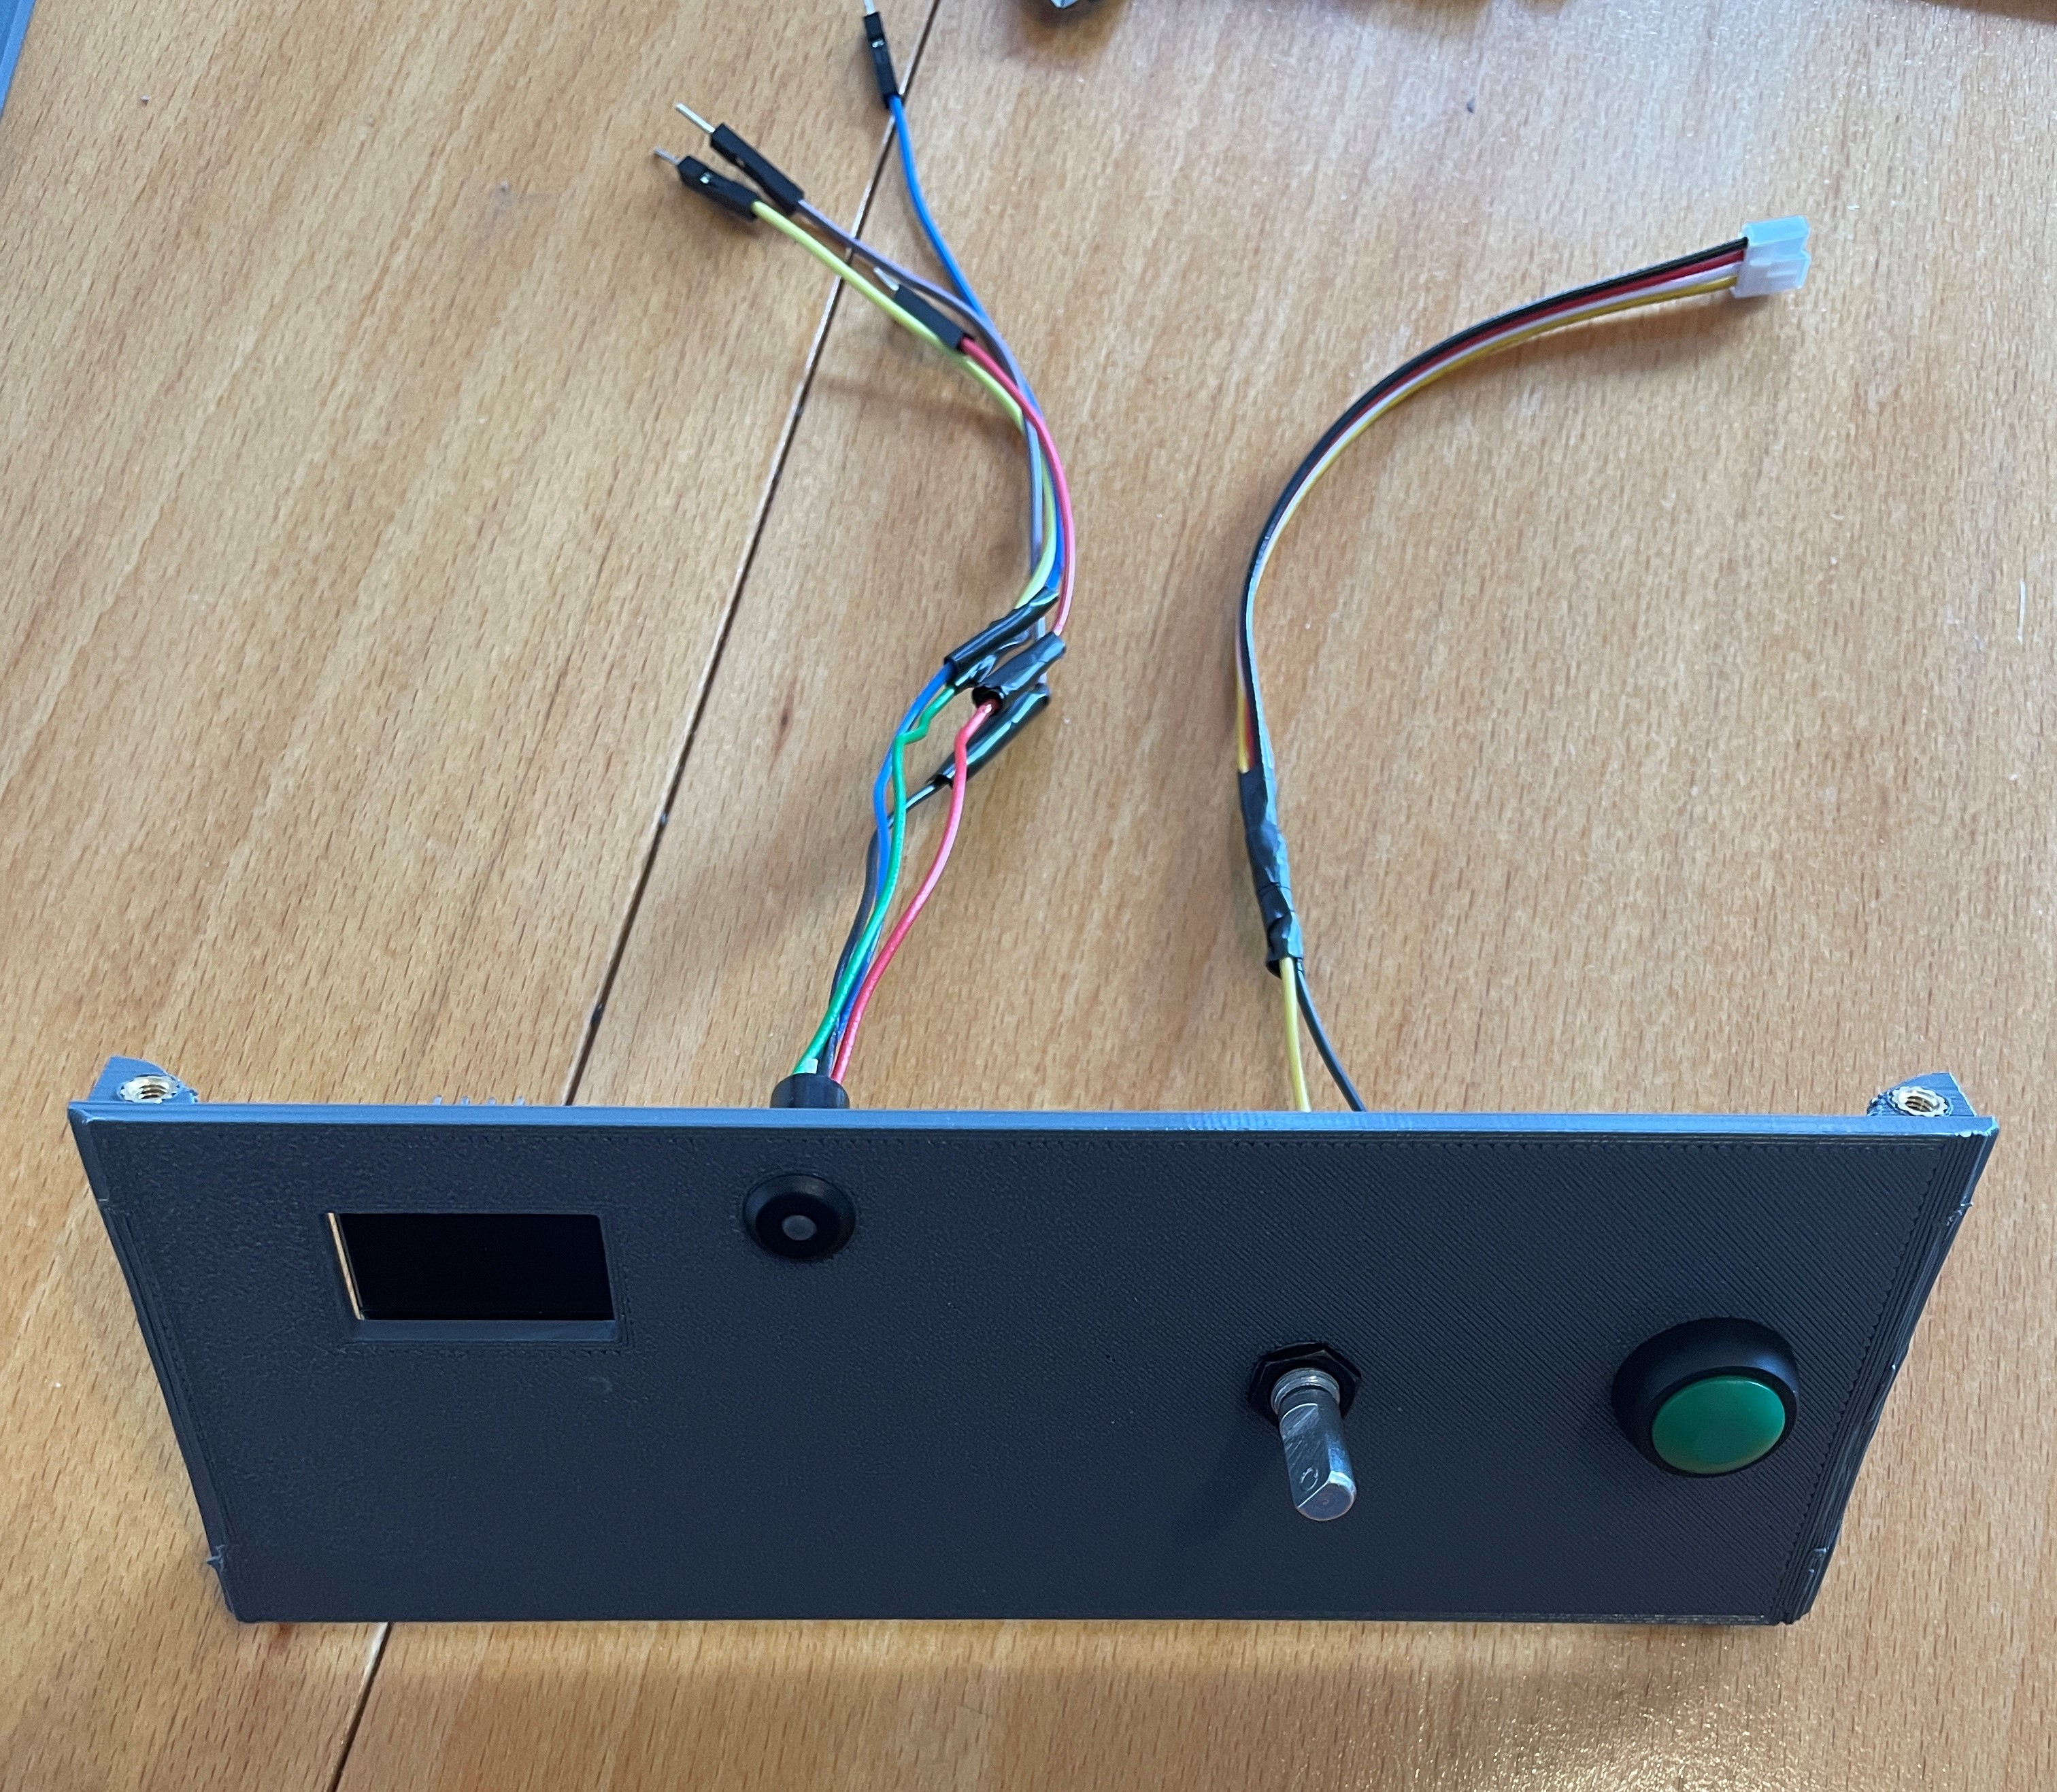
\includegraphics[width=\textwidth]{Images/3Schr.jpg}
		\caption{Dritter Schritt: Zusammenbau der Vorderplatte} \label{3.S}
	\end{center}
\end{figure}


\section{Vierter Schritt: Zusammenbau der Hinterplatte}

Montieren Sie die folgenden Bauteile und elektrischen Komponenten wie in Abbildung \ref{4.S} gezeigt. 

\begin{enumerate}
	\item Montieren Sie den Kaltgeräteanschluss an der Hinterplatte. Ein Klickgeräusch bestätigt den korrekten Sitz.
\end{enumerate}

\begin{figure}[H]
	\begin{center}
		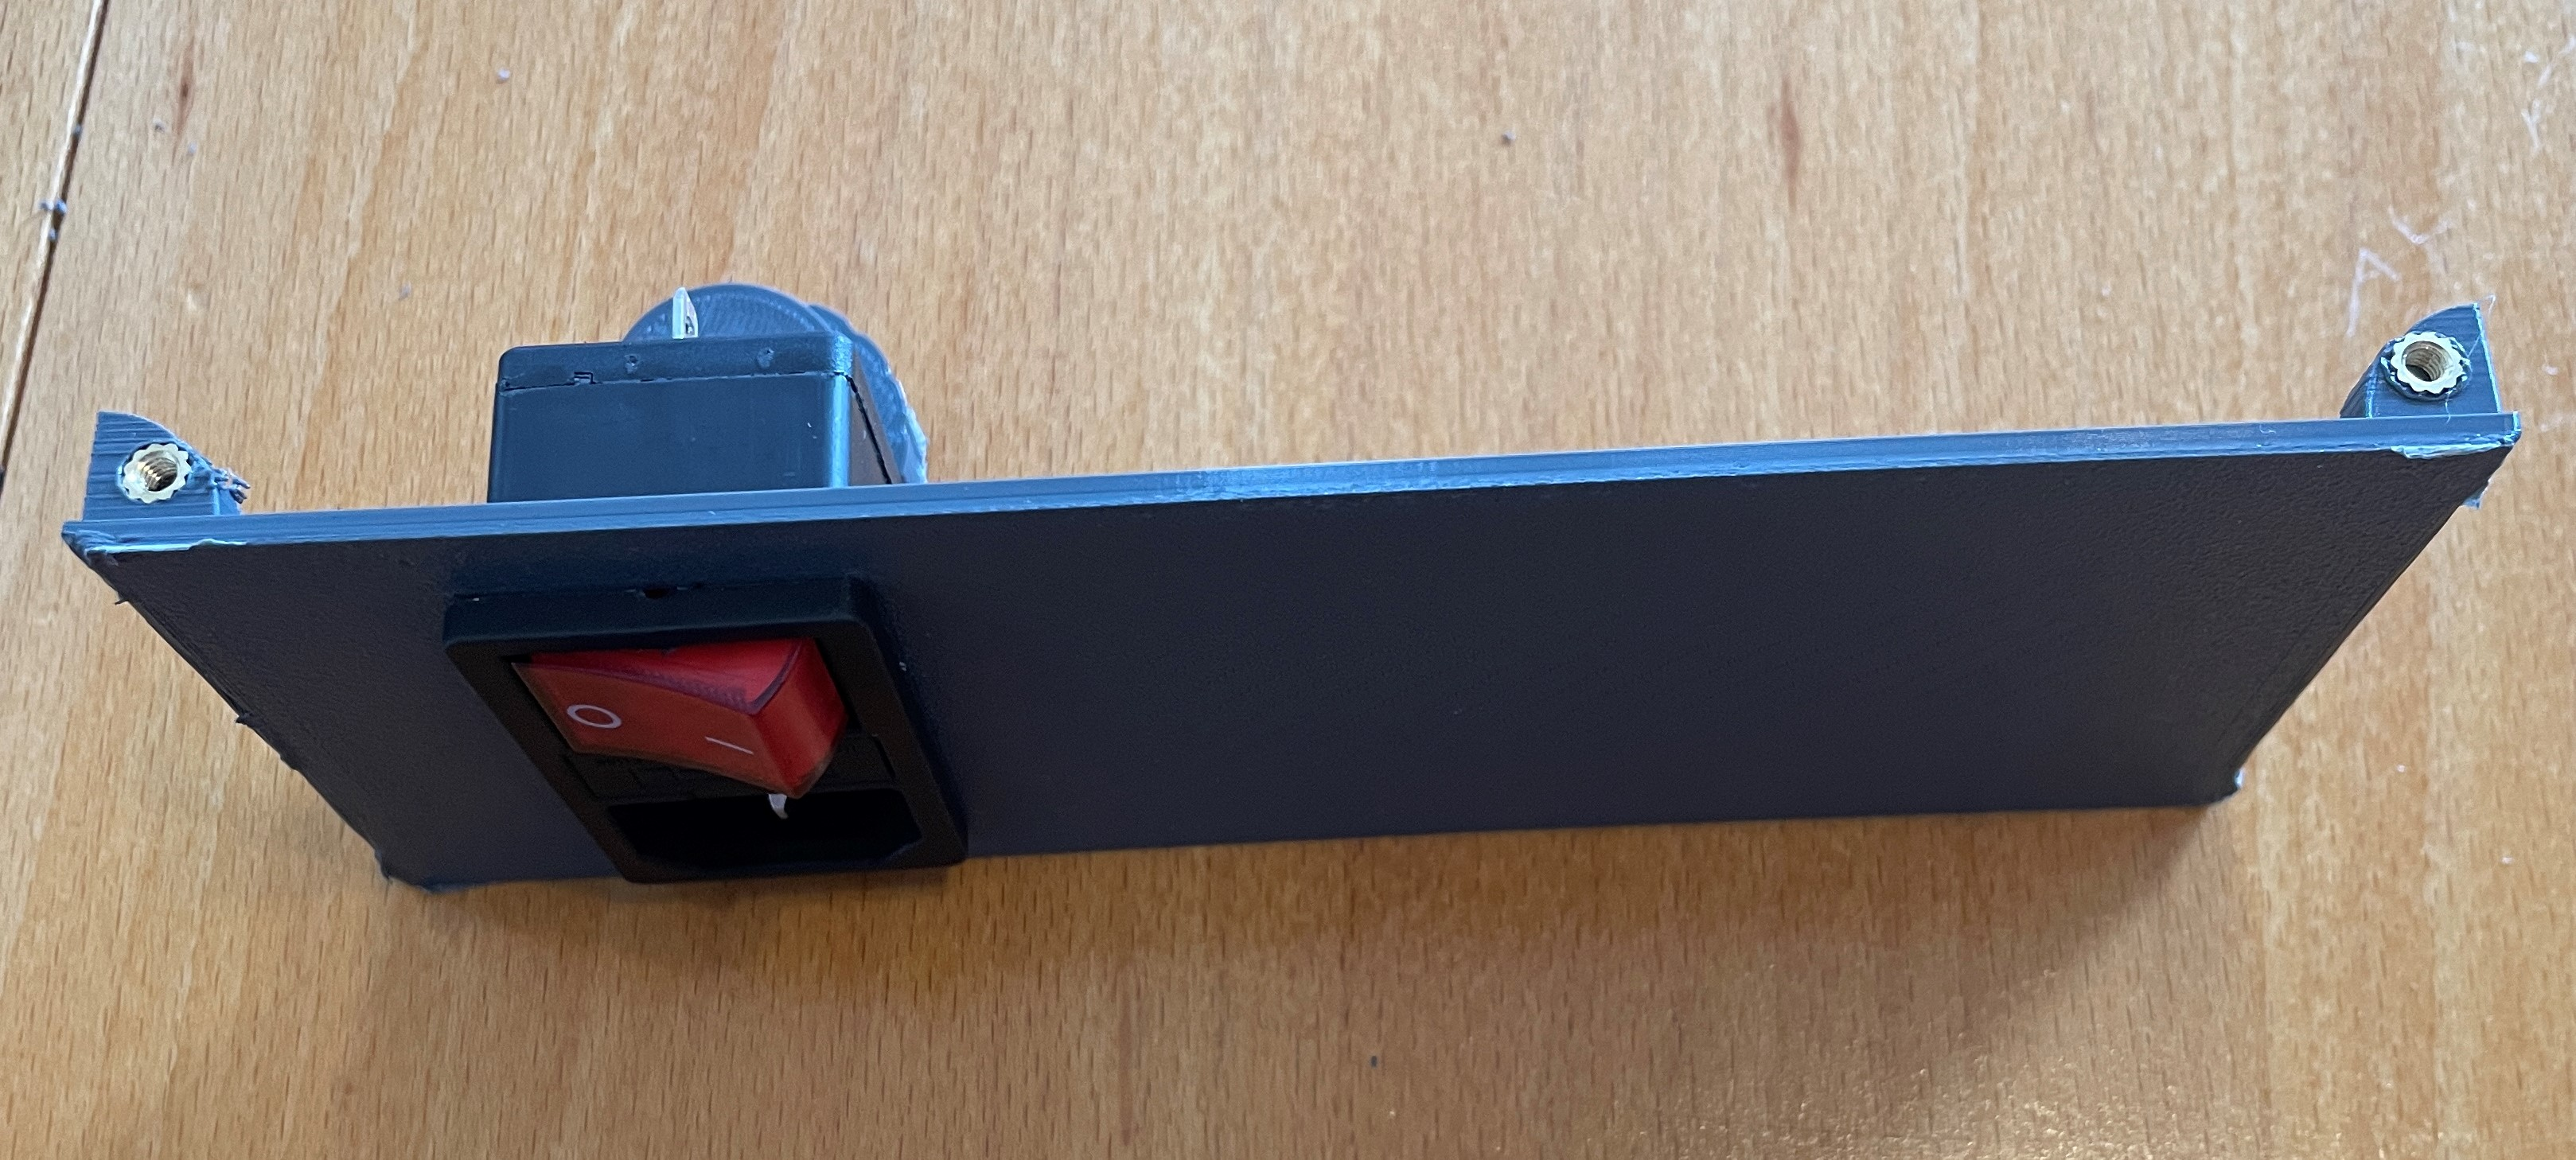
\includegraphics[width=\textwidth]{Images/4Schr.jpg}
		\caption{Vierter Schritt: Zusammenbau der Hinterplatte} \label{4.S}
	\end{center}
\end{figure}


\section{Fünfter Schritt: Teilzusammenbau des Gehäuses}

Montieren Sie die folgenden Bauteile und elektrischen Komponenten wie in Abbildung \ref{5.S} gezeigt. 

\begin{enumerate}
	\item Verschrauben Sie die Vorderplatte und die Hinterplatte mit der Bodenplatte. Verwenden Sie dafür 4 $\times$ $ M3 \times 10 \ mm $ Schrauben.
	\item Befestigen Sie die rechte Seitenplatte mit der Vorder- und Hinterplatte. Verwenden Sie dafür 2 $\times$ $ M3 \times 10 \ mm $ Schrauben.
\end{enumerate}

\begin{figure}[H]
	\begin{center}
		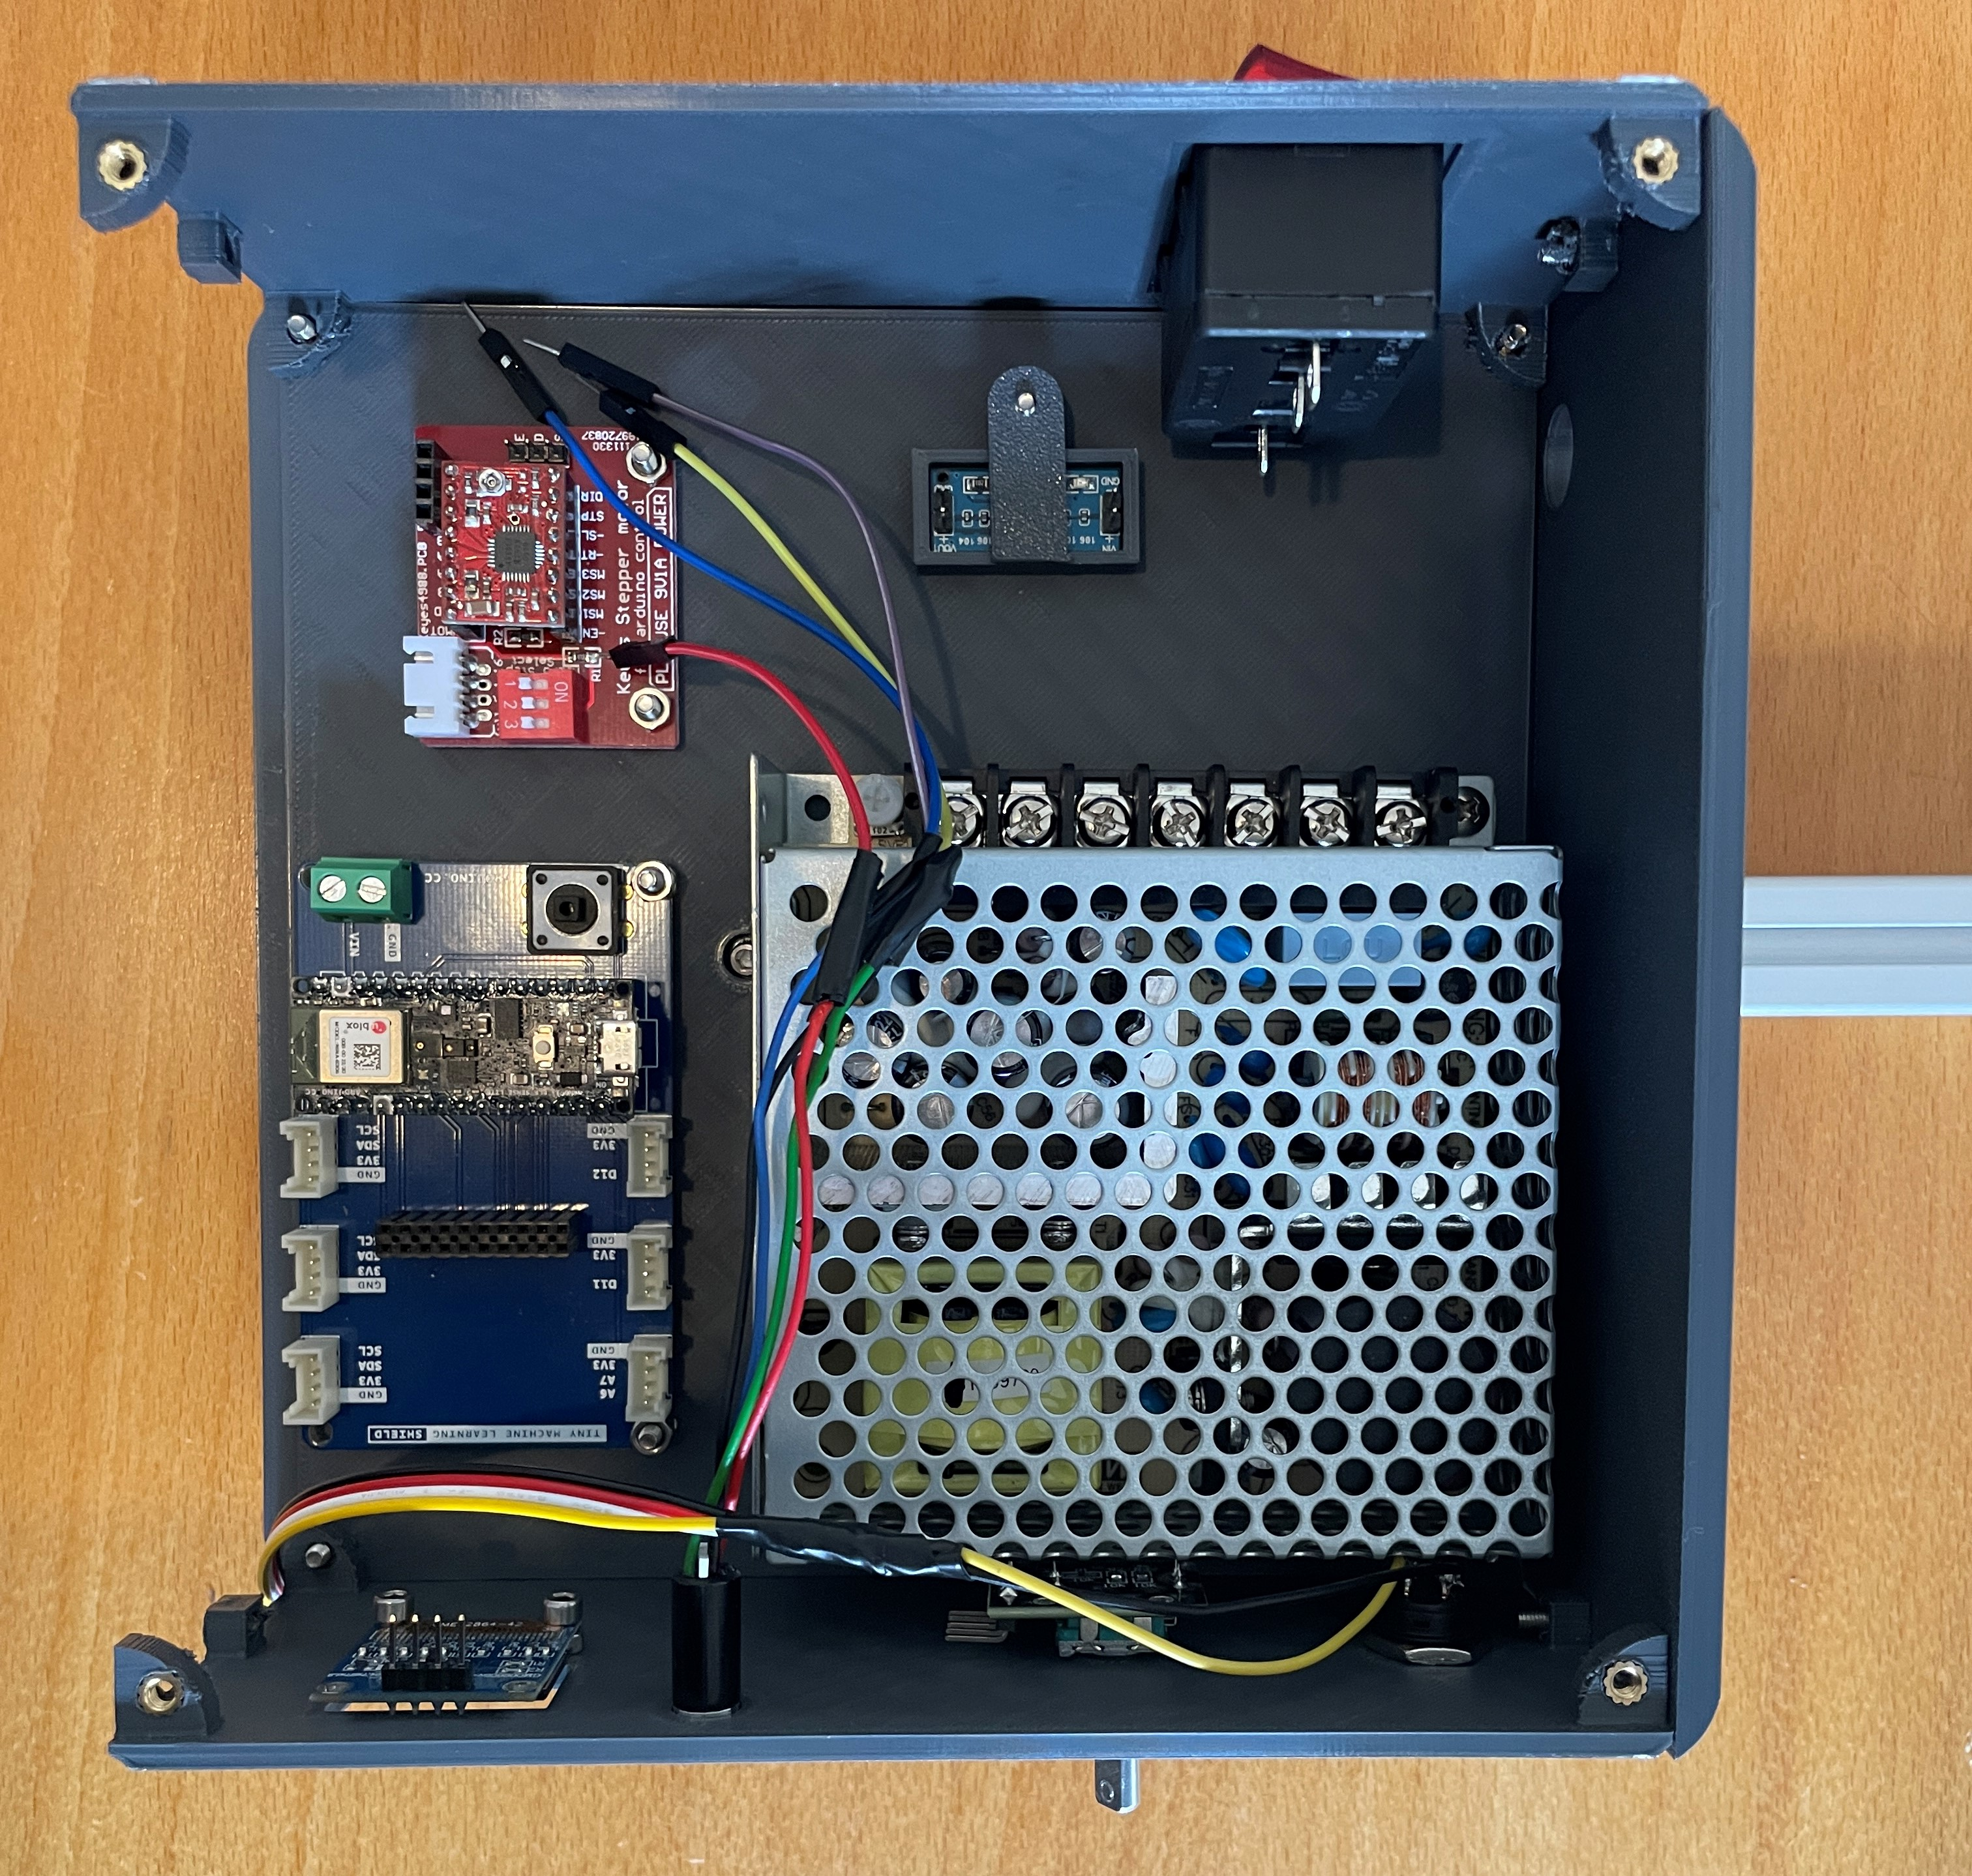
\includegraphics[width=\textwidth]{Images/5Schr.jpg}
		\caption{Fünfter Schritt: Teilzusammenbau des Gehäuses} \label{5.S}
	\end{center}
\end{figure}


\section{Sechster Schritt: Anschließen der elektrischen Leitungen}

\begin{enumerate}
	\item Verbinden Sie die Leitungen gemäß dem Schaltplan (siehe Abbildung \ref{Splan}). Dieser Schritt sollte von einer Elektrofachkraft durchgeführt oder überprüft werden.
	\item Führen Sie die Leitungen für den Motor und den Micro-Schalter durch die Öffnung in der rechten Seitenplatte.
\end{enumerate}

\begin{figure}[H]
	\begin{center}
		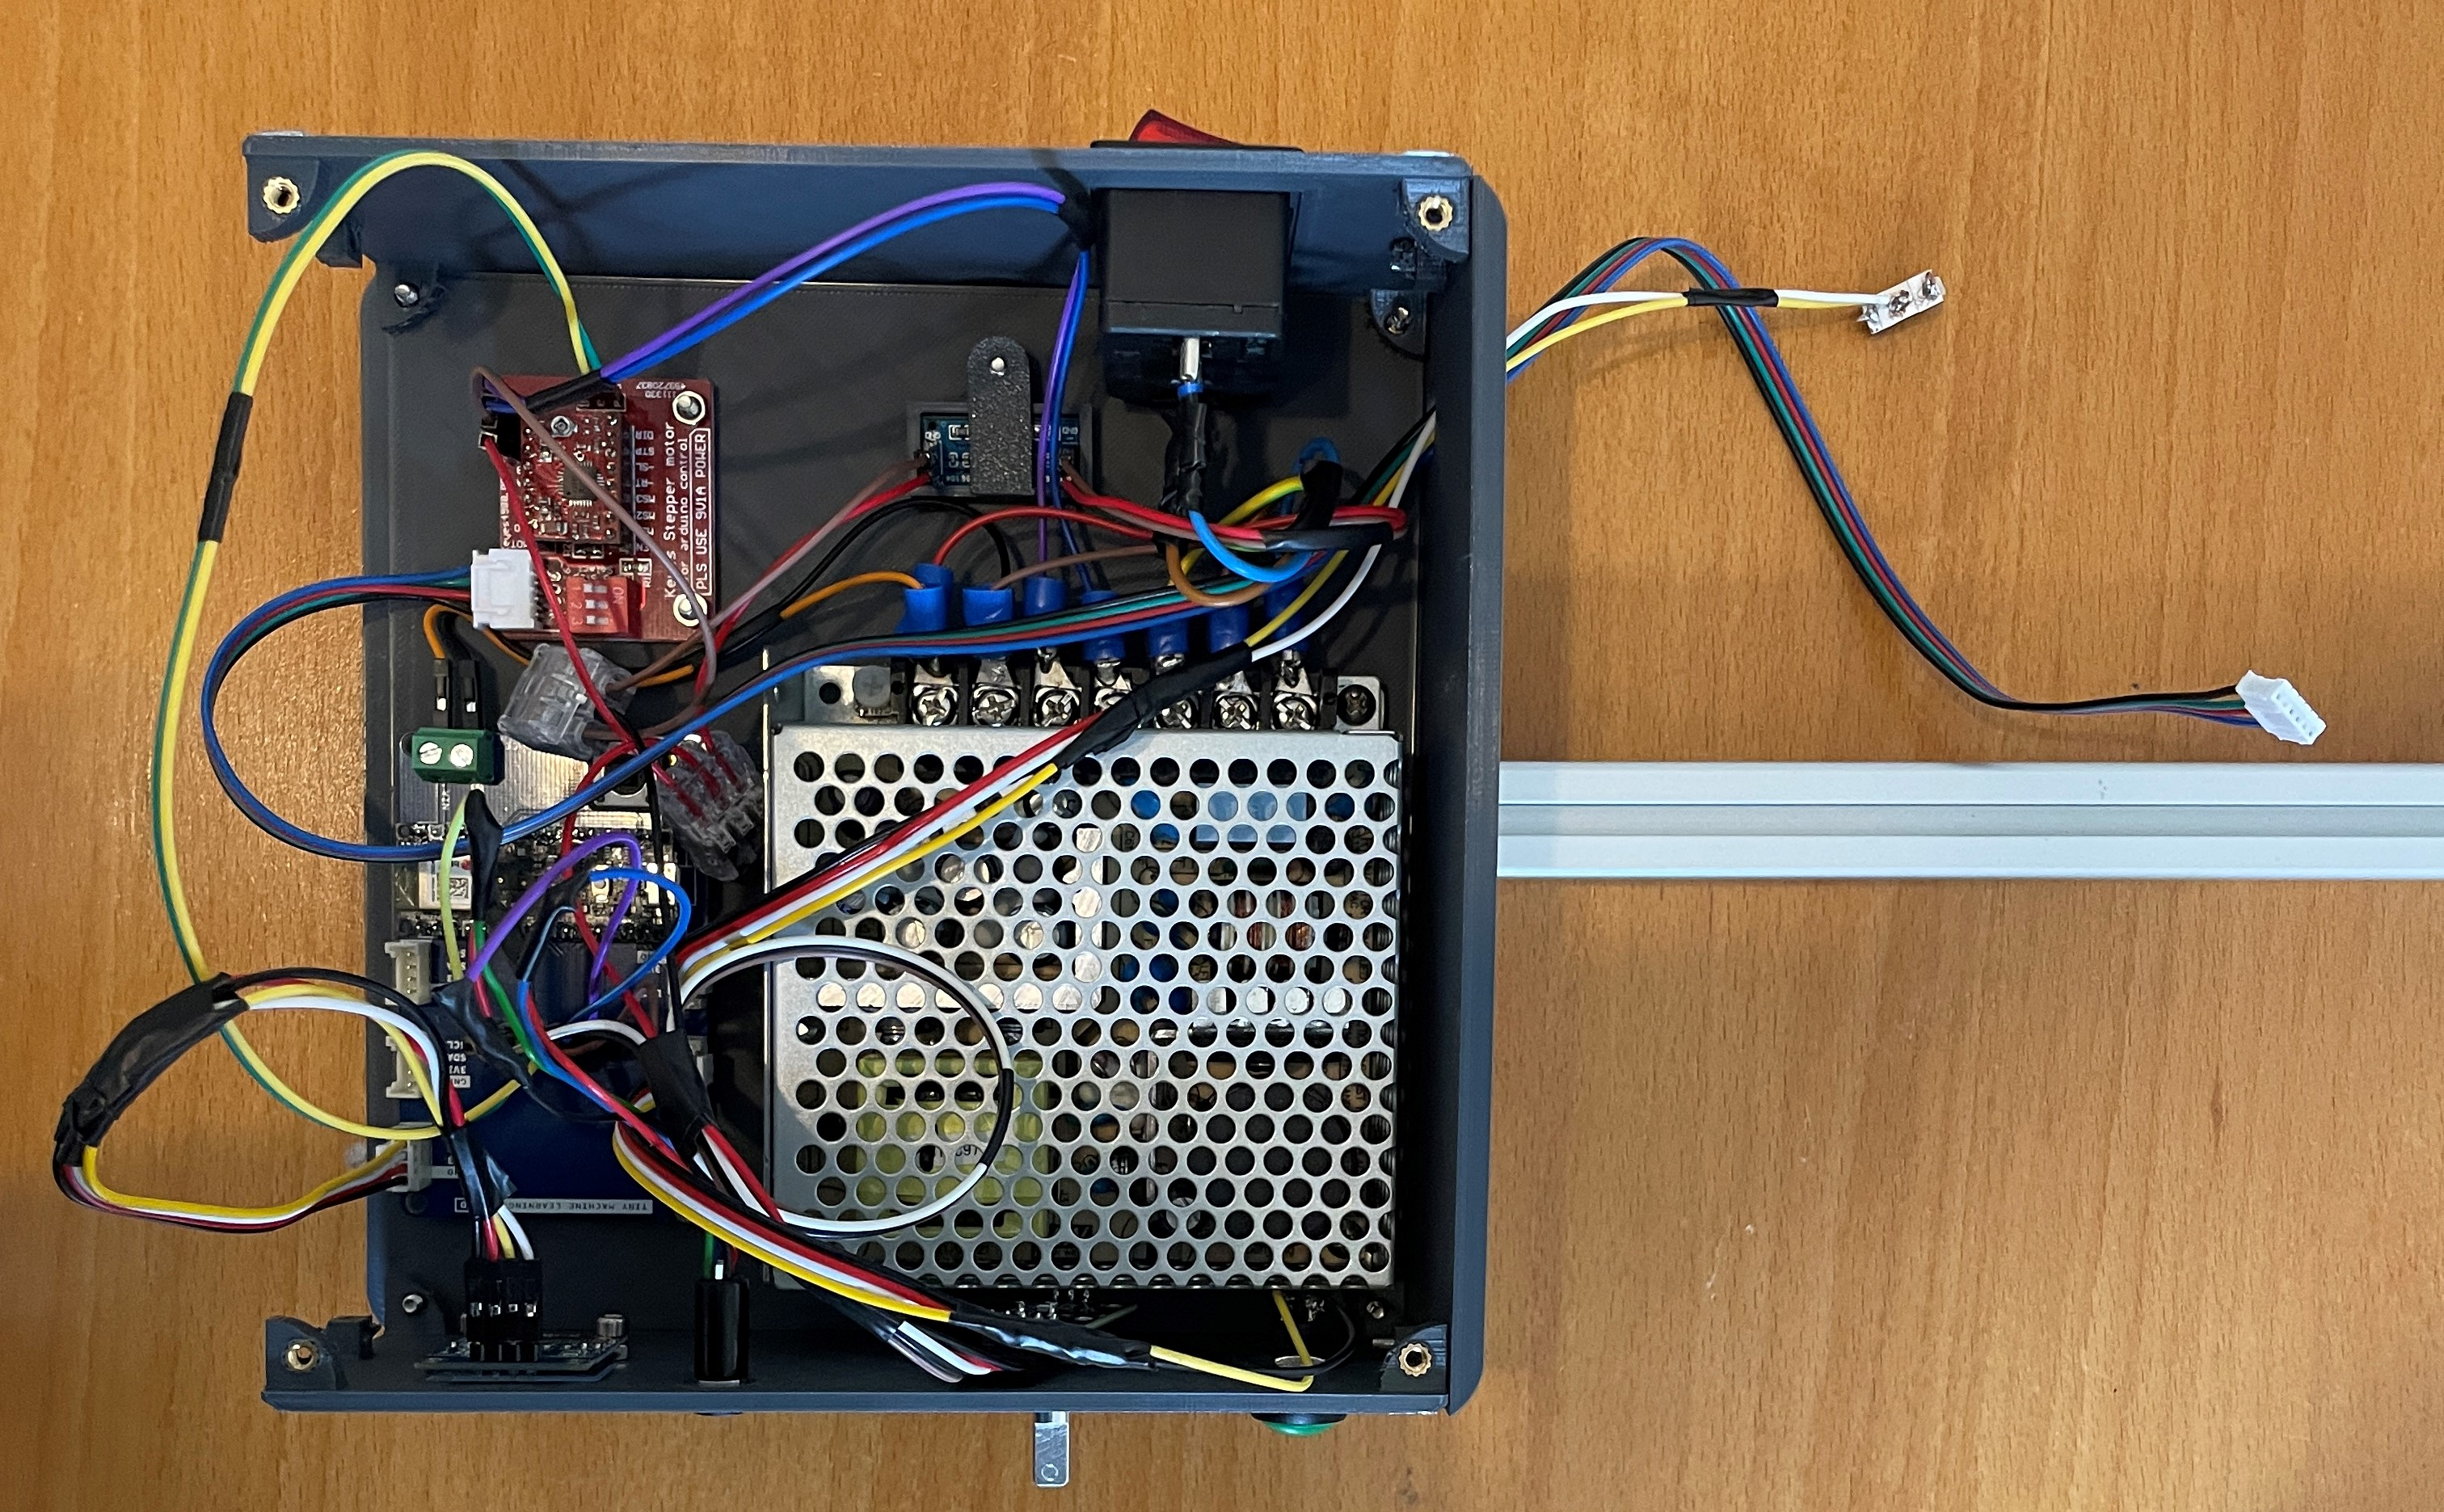
\includegraphics[width=\textwidth]{Images/6Schr.jpg}
		\caption{Schaltplan} \label{6.S}
	\end{center}
\end{figure}


\section{Siebter Schritt: Montieren des Micro-Schalters und Motors}

Montieren Sie die folgenden Bauteile und elektrischen Komponenten wie in Abbildung \ref{7.S} gezeigt.

\begin{enumerate}
	\item Befestigen Sie den Micro-Schalter mit 2 $\times$ $ M2.5 \times 6 \ mm $ Schrauben an der Halterung für den Motor.
	\item Montieren Sie den Nema 17 Motor an der Halterung für die Welle mit 4 $\times$ $ M3 \times 6 \ mm  $ Schrauben.
	\item Führen Sie 2 $\times$ $ M3 $ Hammermutter in das Aluprofil ein.
	\item Befestigen Sie die Halterung am Aluprofil mit 2 $\times$ $ M3 \times 8 \ mm $ und 2 $\times$ $ M3 $ Hammermuttern. Halten Sie einen Abstand vom Gehäuse von ca. 15 bis 20 \ mm. 
	\item Verbinden Sie die Leitung für den Motor an dem Motor. 
\end{enumerate}

\begin{figure}[H]
	\begin{center}
		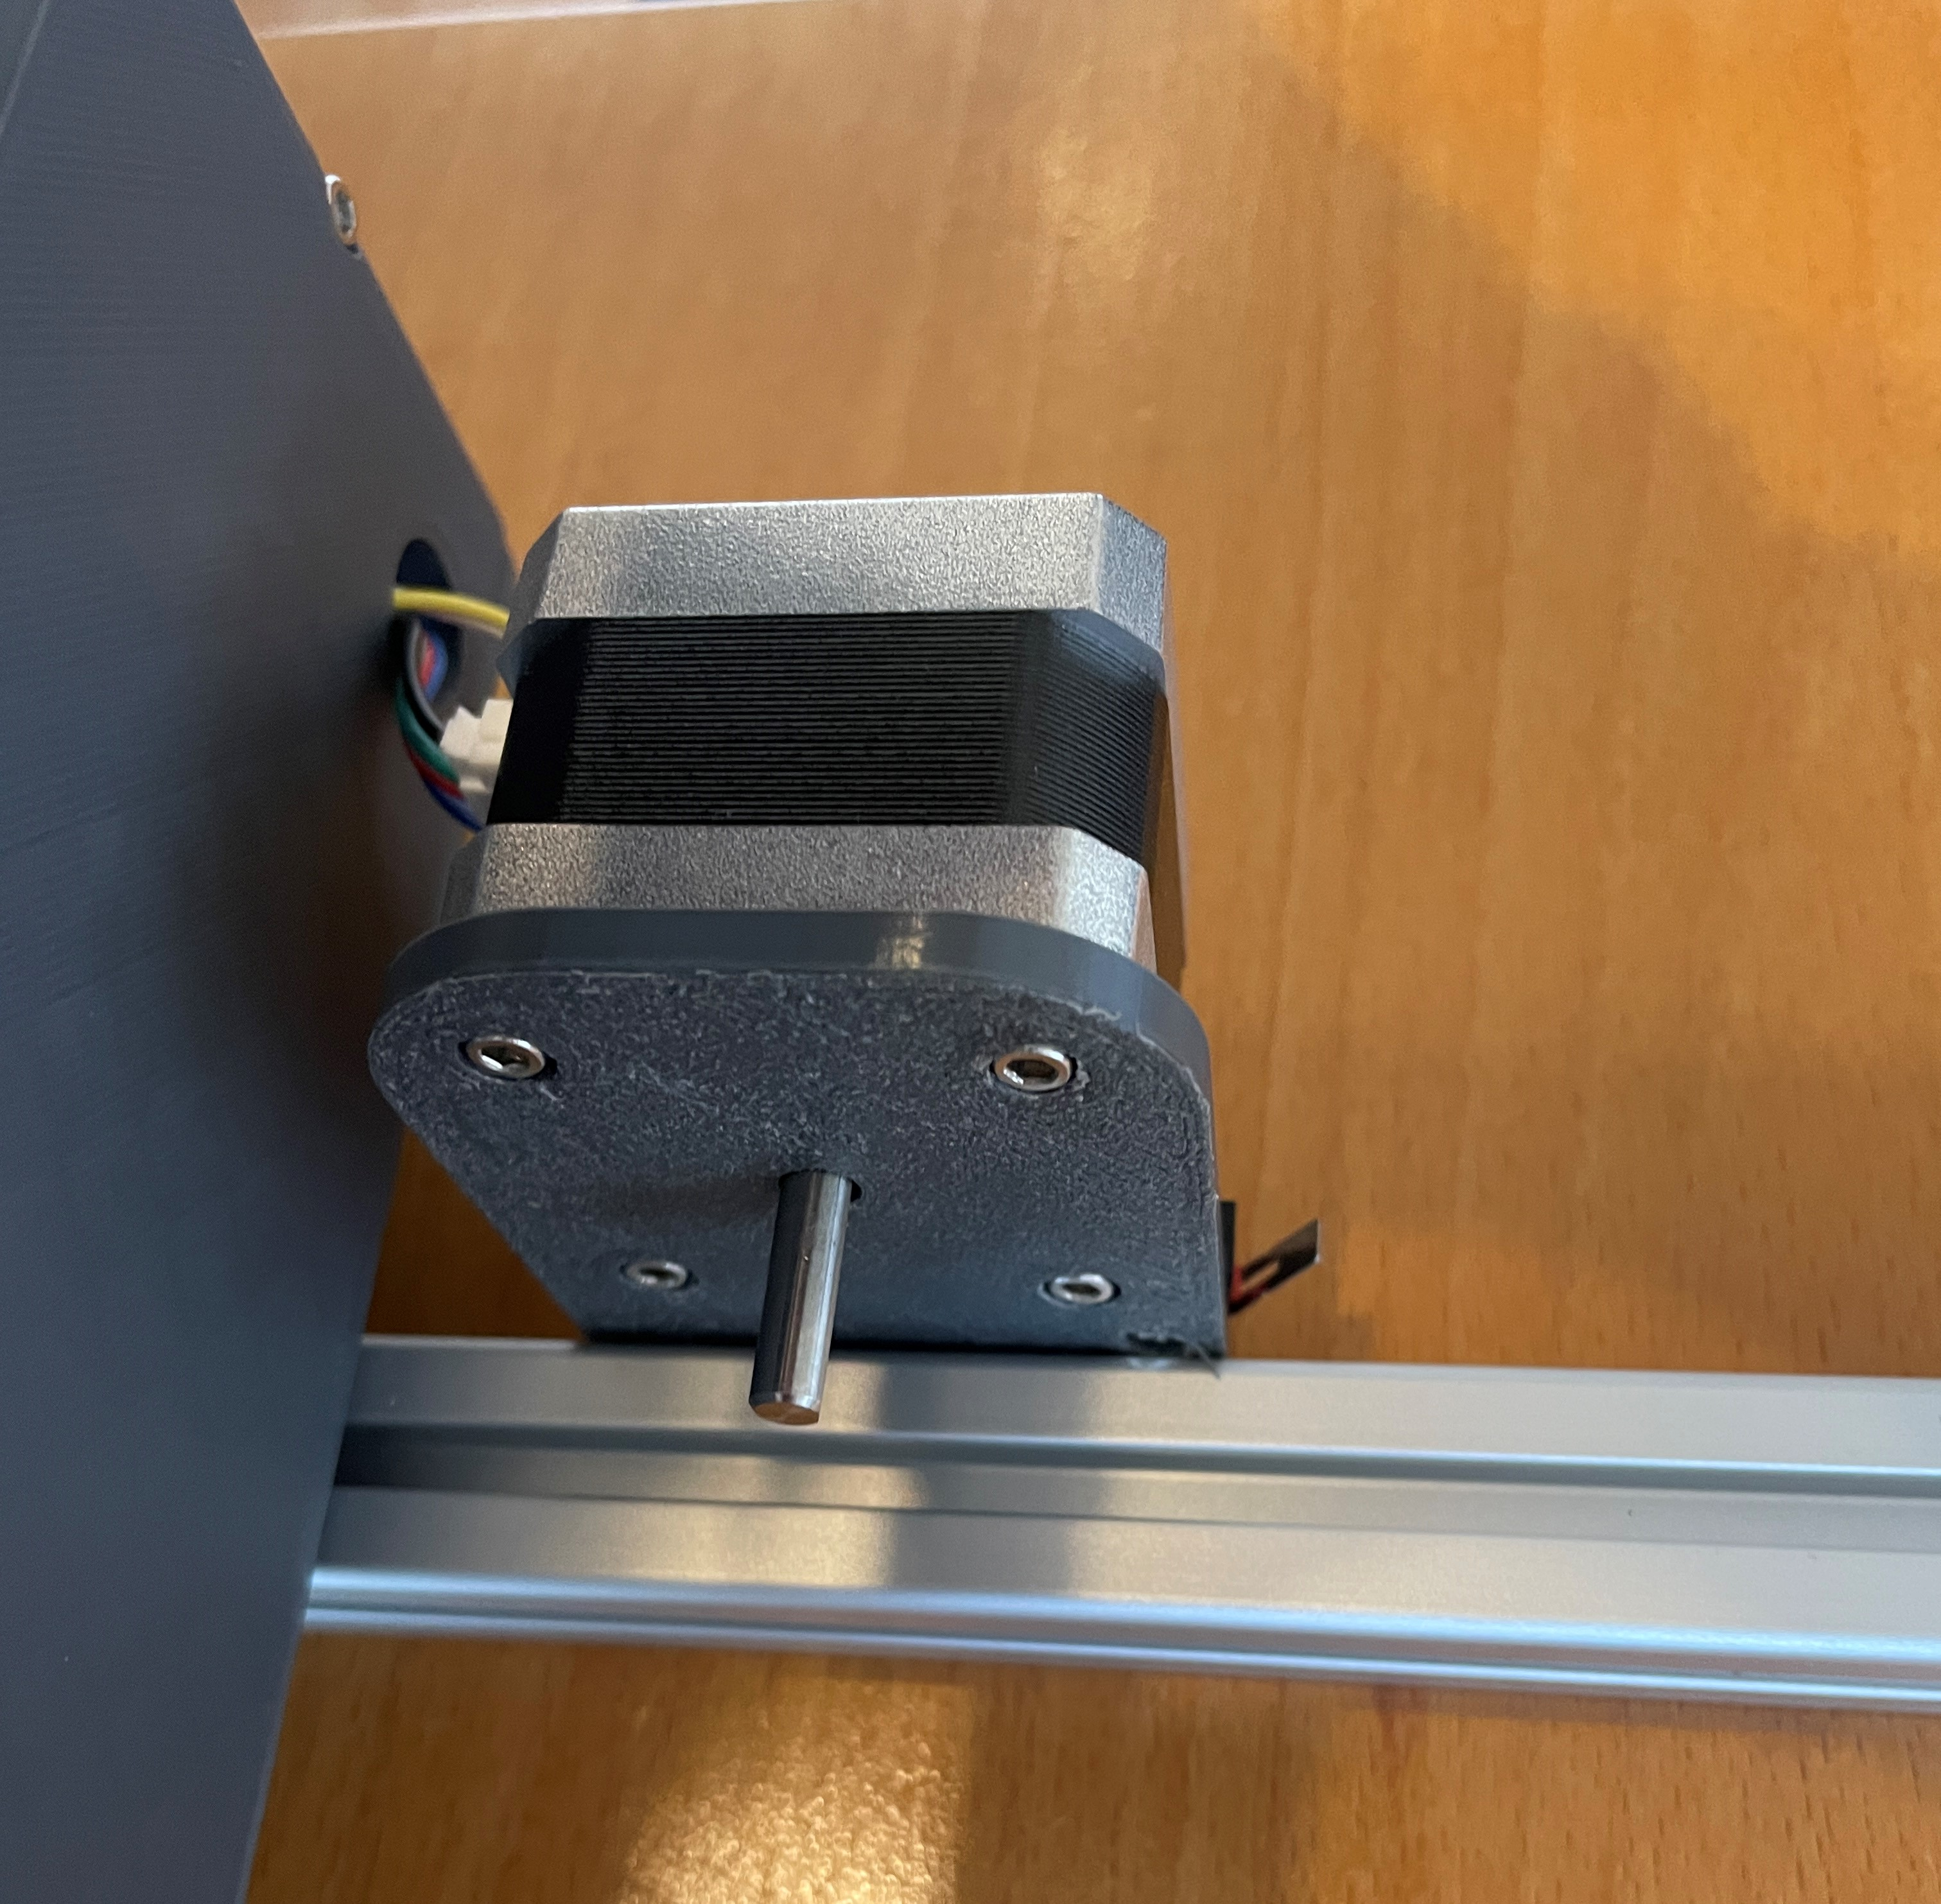
\includegraphics[width=\textwidth]{Images/7Schr.jpg}
		\caption{Siebter Schritt: Montieren des Micro-Schalters und Motors} \label{7.S}
	\end{center}
\end{figure}


\section{Achter Schritt: Zusammenbau des Gehäuses}

Montieren Sie die folgenden Bauteile und elektrischen Komponenten wie in Abbildung \ref{8.S} gezeigt.

\begin{enumerate}
	\item Verschrauben Sie die Seitenplatte Links und die Hinterplatte mit der Vorderplatte und Hinterplatte. Verwenden Sie dafür 2 $\times$ $ M3 \times 10 \ mm $ Schrauben.
	\item Verschrauben Sie die Deckelplatte mit der Vorderplatte und Hinterplatte. Verwenden Sie dafür 4 $\times$ $ M3 \times 10 \ mm $ Schrauben.
\end{enumerate}

\begin{figure}[H]
	\begin{center}
		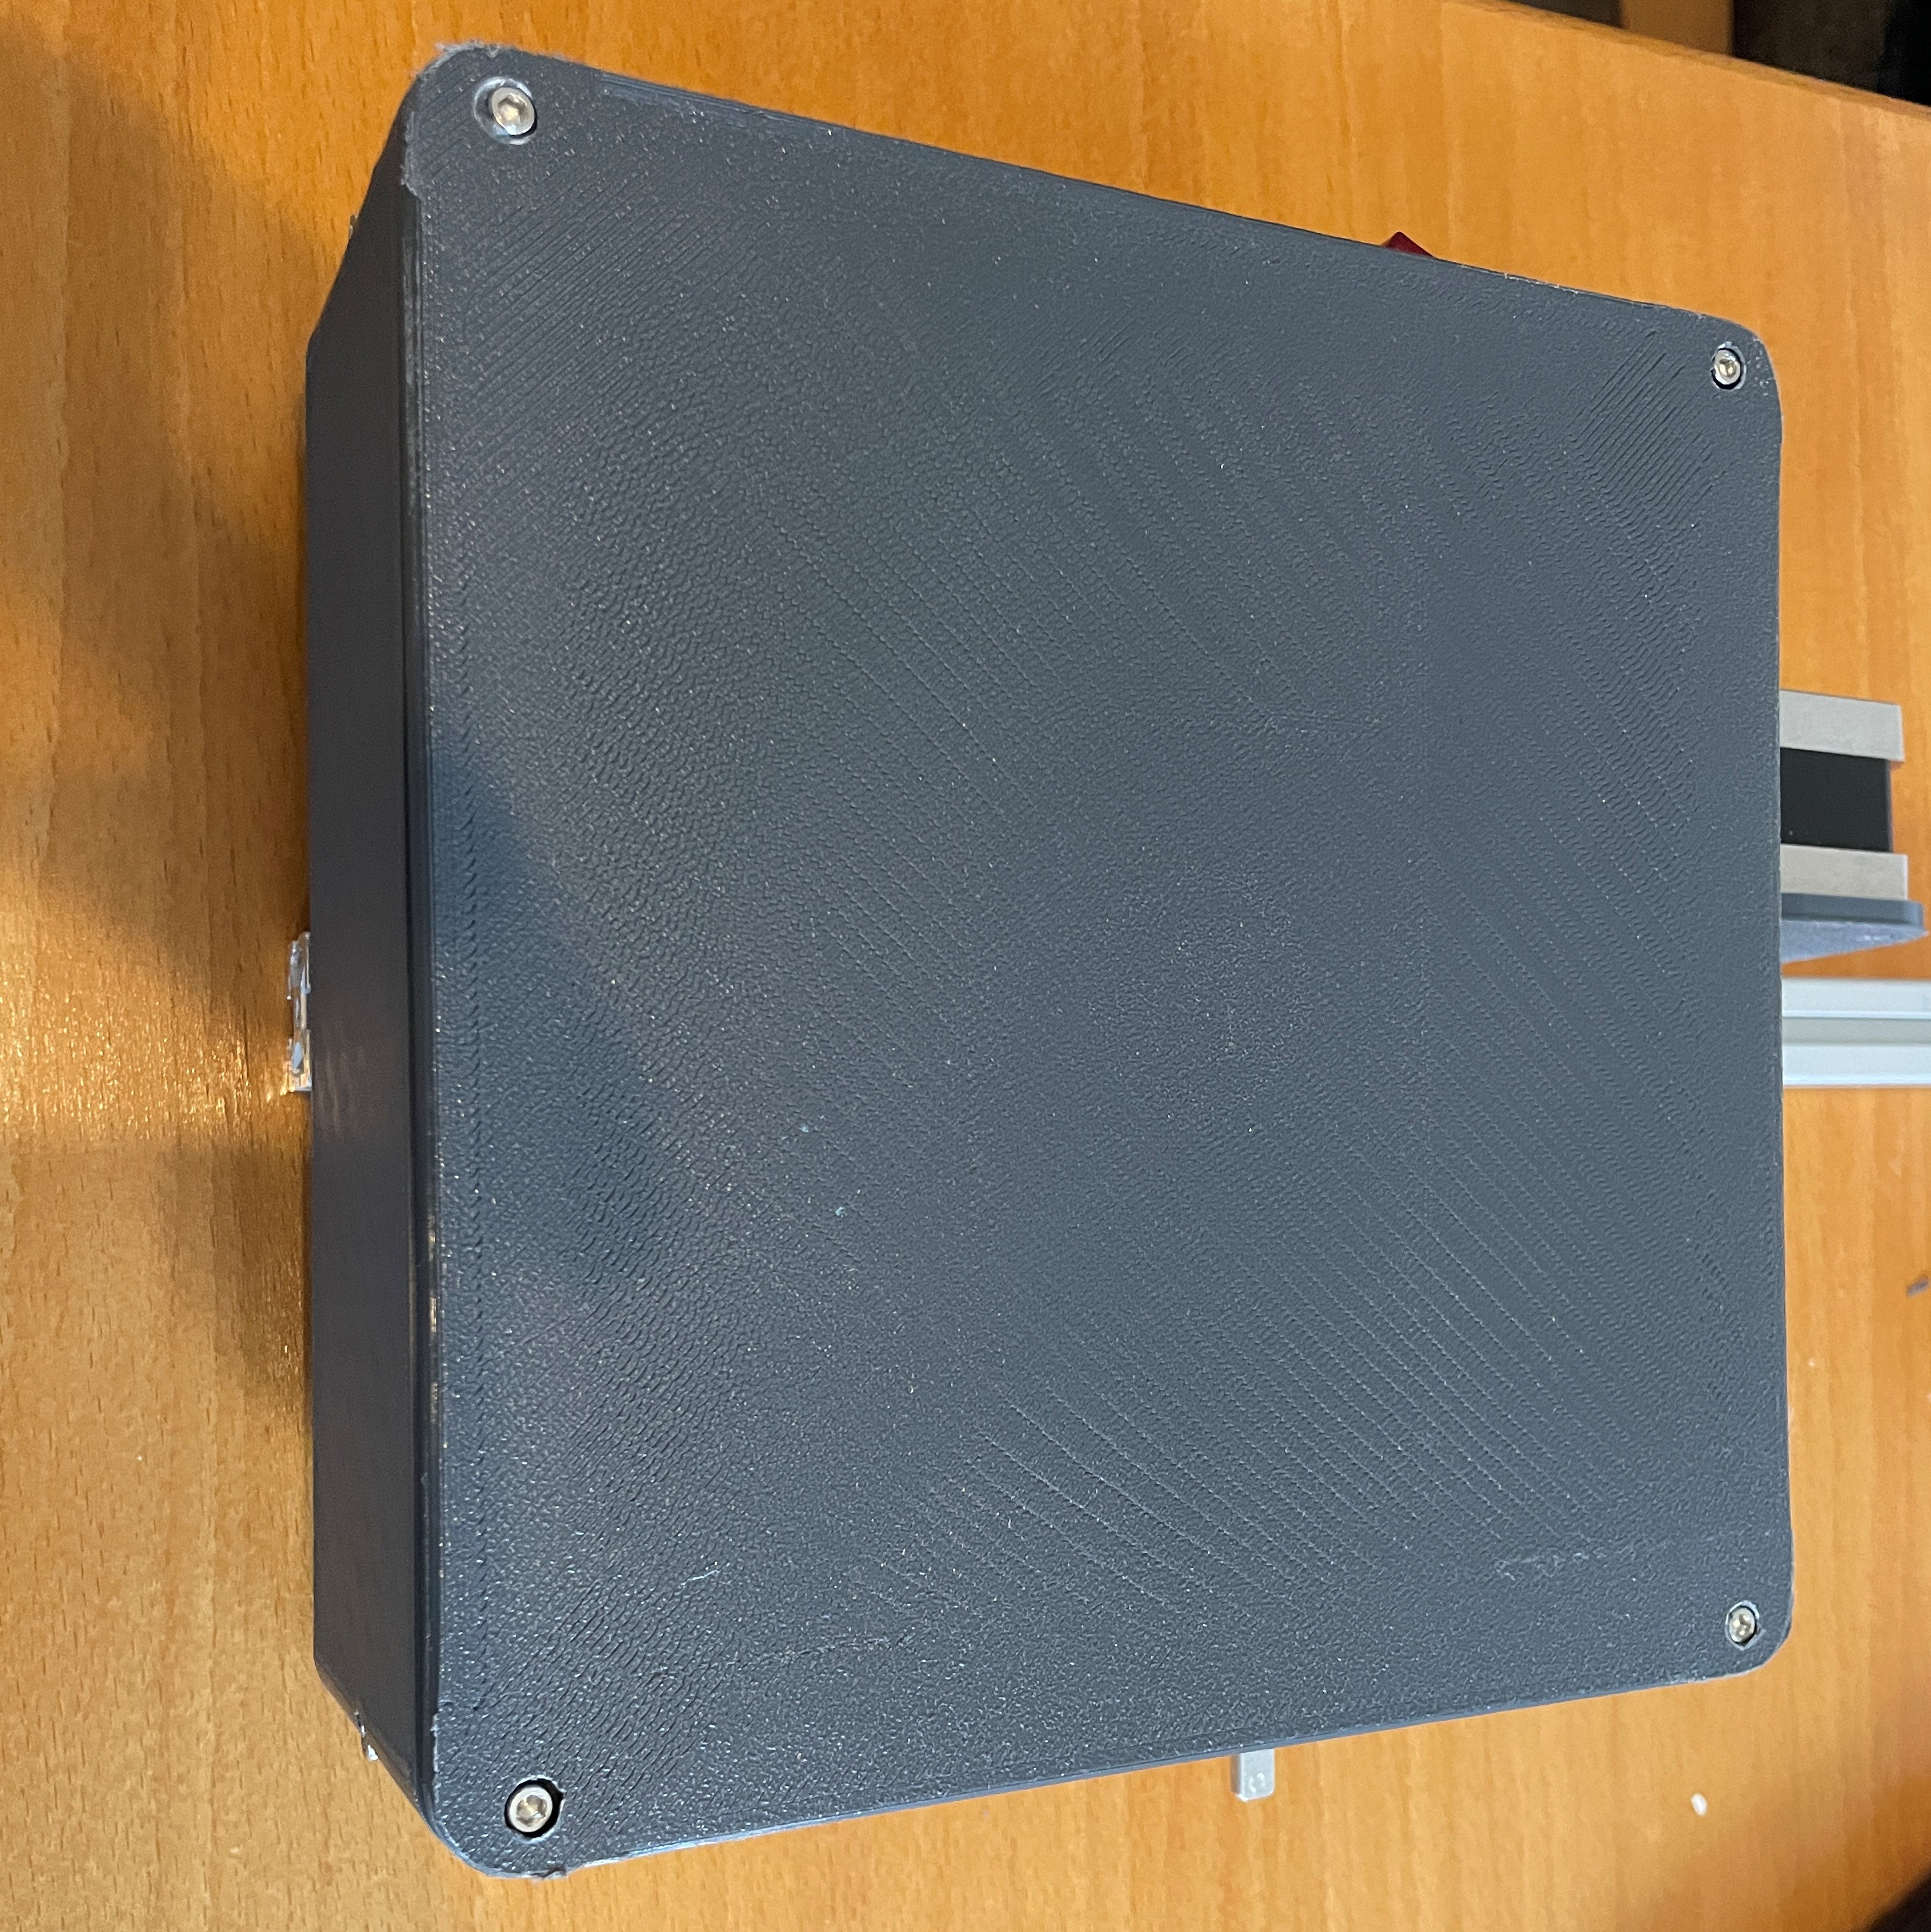
\includegraphics[width=\textwidth]{Images/8Schr.jpg}
		\caption{Achter Schritt: Zusammenbau des Gehäuses} \label{8.S}
	\end{center}
\end{figure}

\section{Neunter Schritt: Montieren der Linearführung}

Montieren Sie die folgenden Bauteile wie in Abbildung \ref{9.S} gezeigt.

\begin{enumerate}
	\item Führen Sie 5 $\times$ $ M3 $ Hammermutter in das Aluprofil ein.
	\item Befestigen Sie die Liniearführung am Aluprofil mit 5 $\times$ $ M3 \times 10 \ mm $ und 5 $\times$ $ M3 $ Hammermuttern. Lassen Sie an jeder Seite eine Bohrung frei und nutzen Sie dann jede fünfte Bohrung. 
\end{enumerate}

\begin{figure}[H]
	\begin{center}
		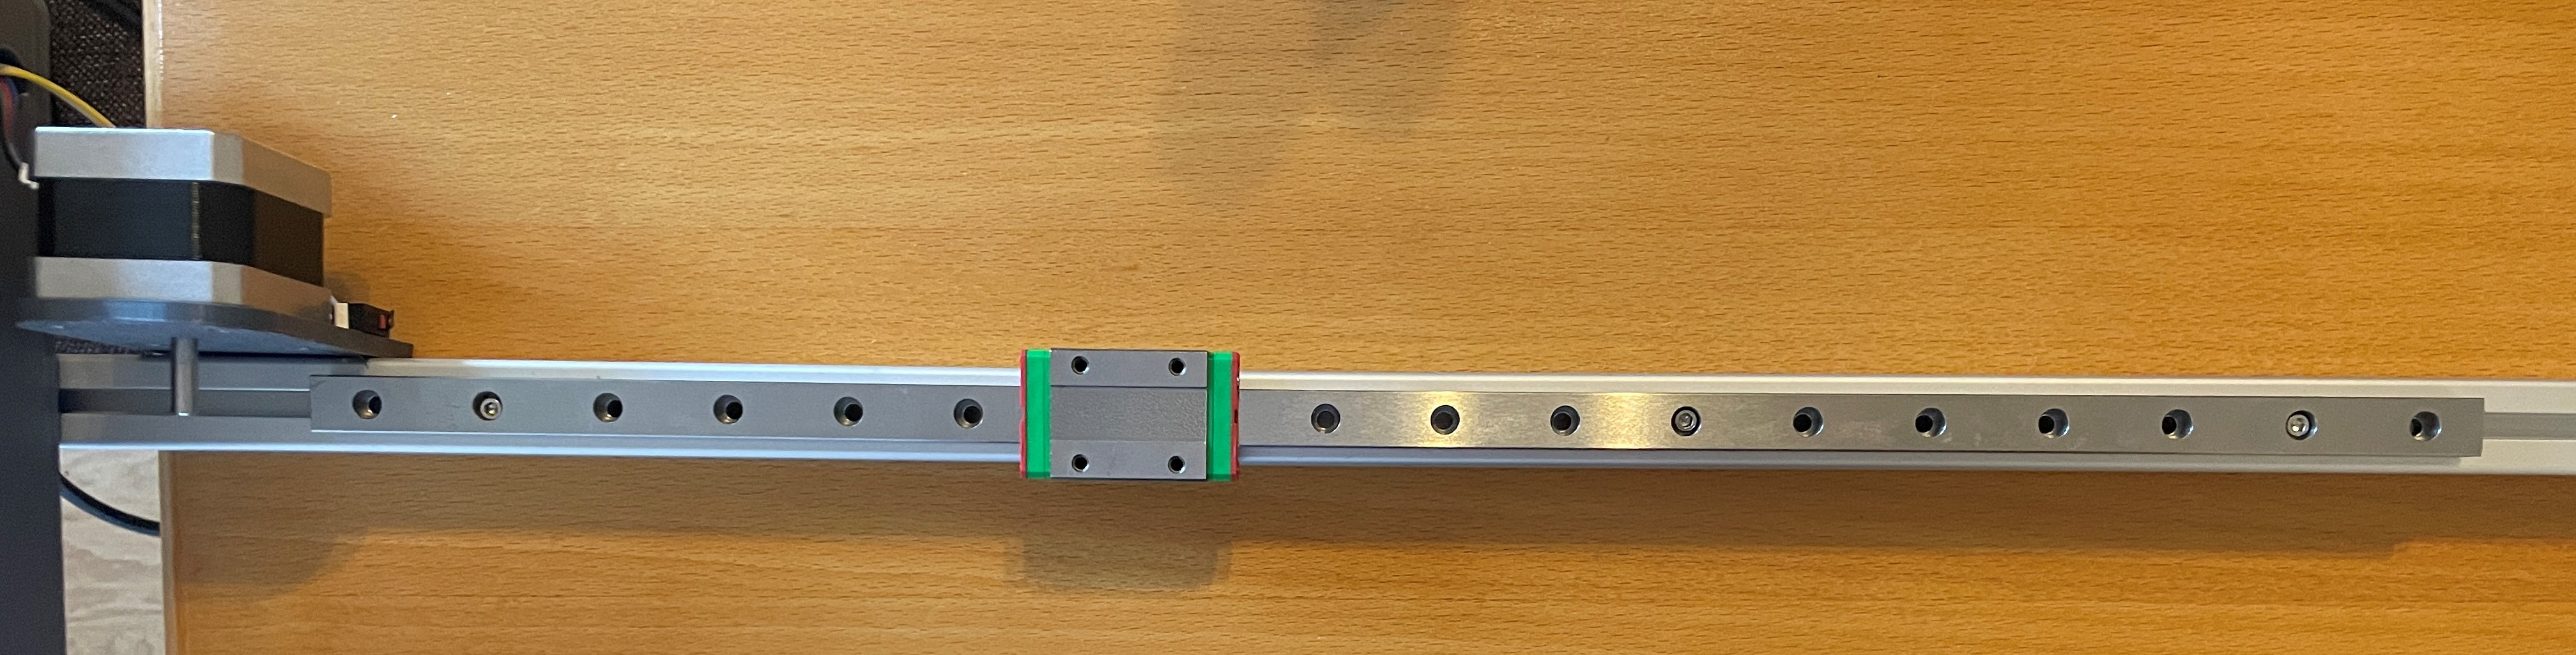
\includegraphics[width=\textwidth]{Images/9Schr.jpg}
		\caption{Neunter Schritt: Montage der Liniearführung} \label{9.S}
	\end{center}
\end{figure}

\section{Zehnter Schritt: Montieren des Griffs}
Montieren Sie die folgenden Bauteile wie in Abbildung \ref{10.S} gezeigt.

\begin{enumerate}
	\item Führen Sie 2 $\times$ $ M3 $ Hammermutter in das Aluprofil ein.
	\item Montieren Sie den Anzeiger auf den Schlitten der Liniearführung mit 4 $\times$ $ M3 \times 6 \ mm $ Schrauben.
	\item Montieren Sie den Riemen Auf den Anzeiger mit 4 $\times$ $ M3 \times 6 \ mm $ Schrauben.
\end{enumerate}

\begin{figure}[H]
	\begin{center}
		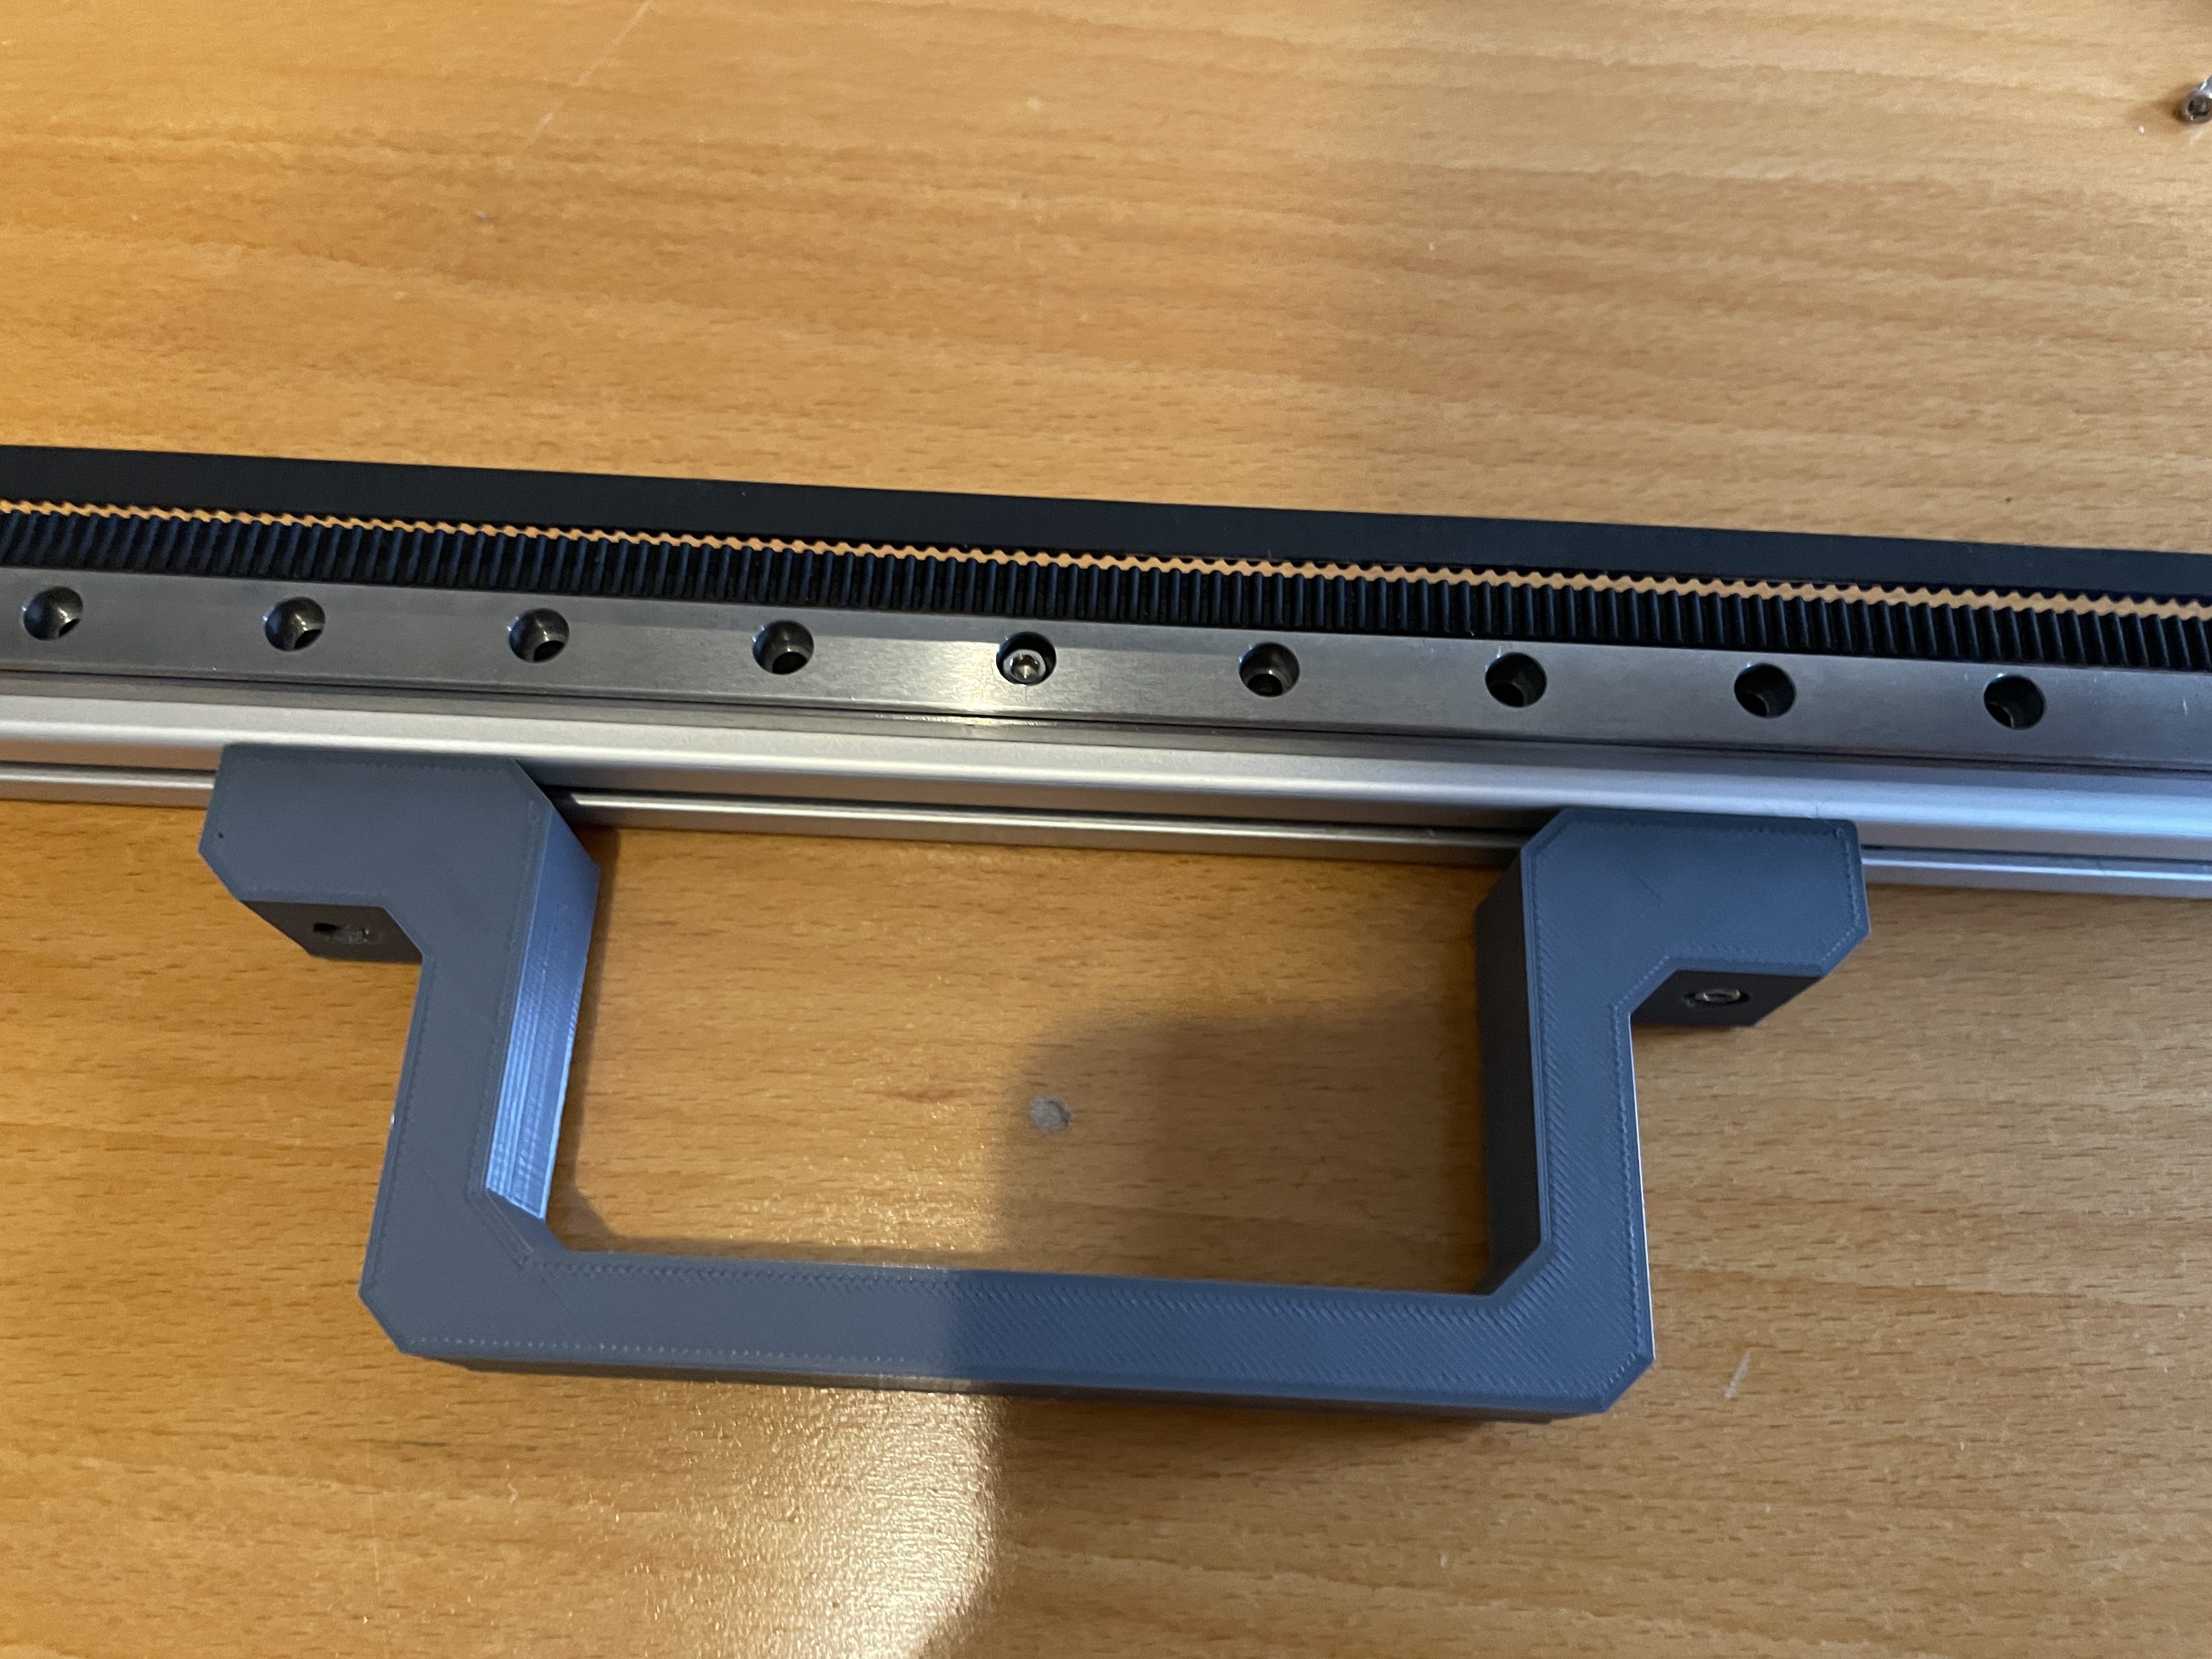
\includegraphics[width=\textwidth]{Images/10Schr.jpg}
		\caption{Dreizehnter Schritt:Montieren des Griffs} \label{10.S}
	\end{center}
\end{figure}


\section{Elfter Schritt: Montieren der Halter für die Welle}

Montieren Sie die folgenden Bauteile wie in Abbildung \ref{11.S} gezeigt.

\begin{enumerate}
	\item Führen Sie jeweils 2 $\times$ $ M3 $ Hammermutter gegenüberliegend in das Aluprofil ein. Führen Sie außerdem 2 $\times$ $ M3 $ Hammermutter an der vorderen Seite für die spätere Montage des Lineals ein. 
	\item Befestigen Sie die erste Halterung am Aluprofil mit 2 $\times$ $ M3 \times 8 \ mm $ und 2 $\times$ $ M3 $ Hammermuttern.
	\item Führen Sie die Welle in die \O 7 \ mm Bohrung der Halterung ein.
	\item Stecken Sie auf die Welle die Riemenscheibe.
	\item Befestigen Sie die zweite Halterung gegenüberliegend der ersten Halterung am Aluprofil mit 2 $\times$ $ M3 \times 8 \ mm $ und 2 $\times$ $ M3 $ Hammermuttern.
\end{enumerate}

\begin{figure}[H]
	\begin{center}
		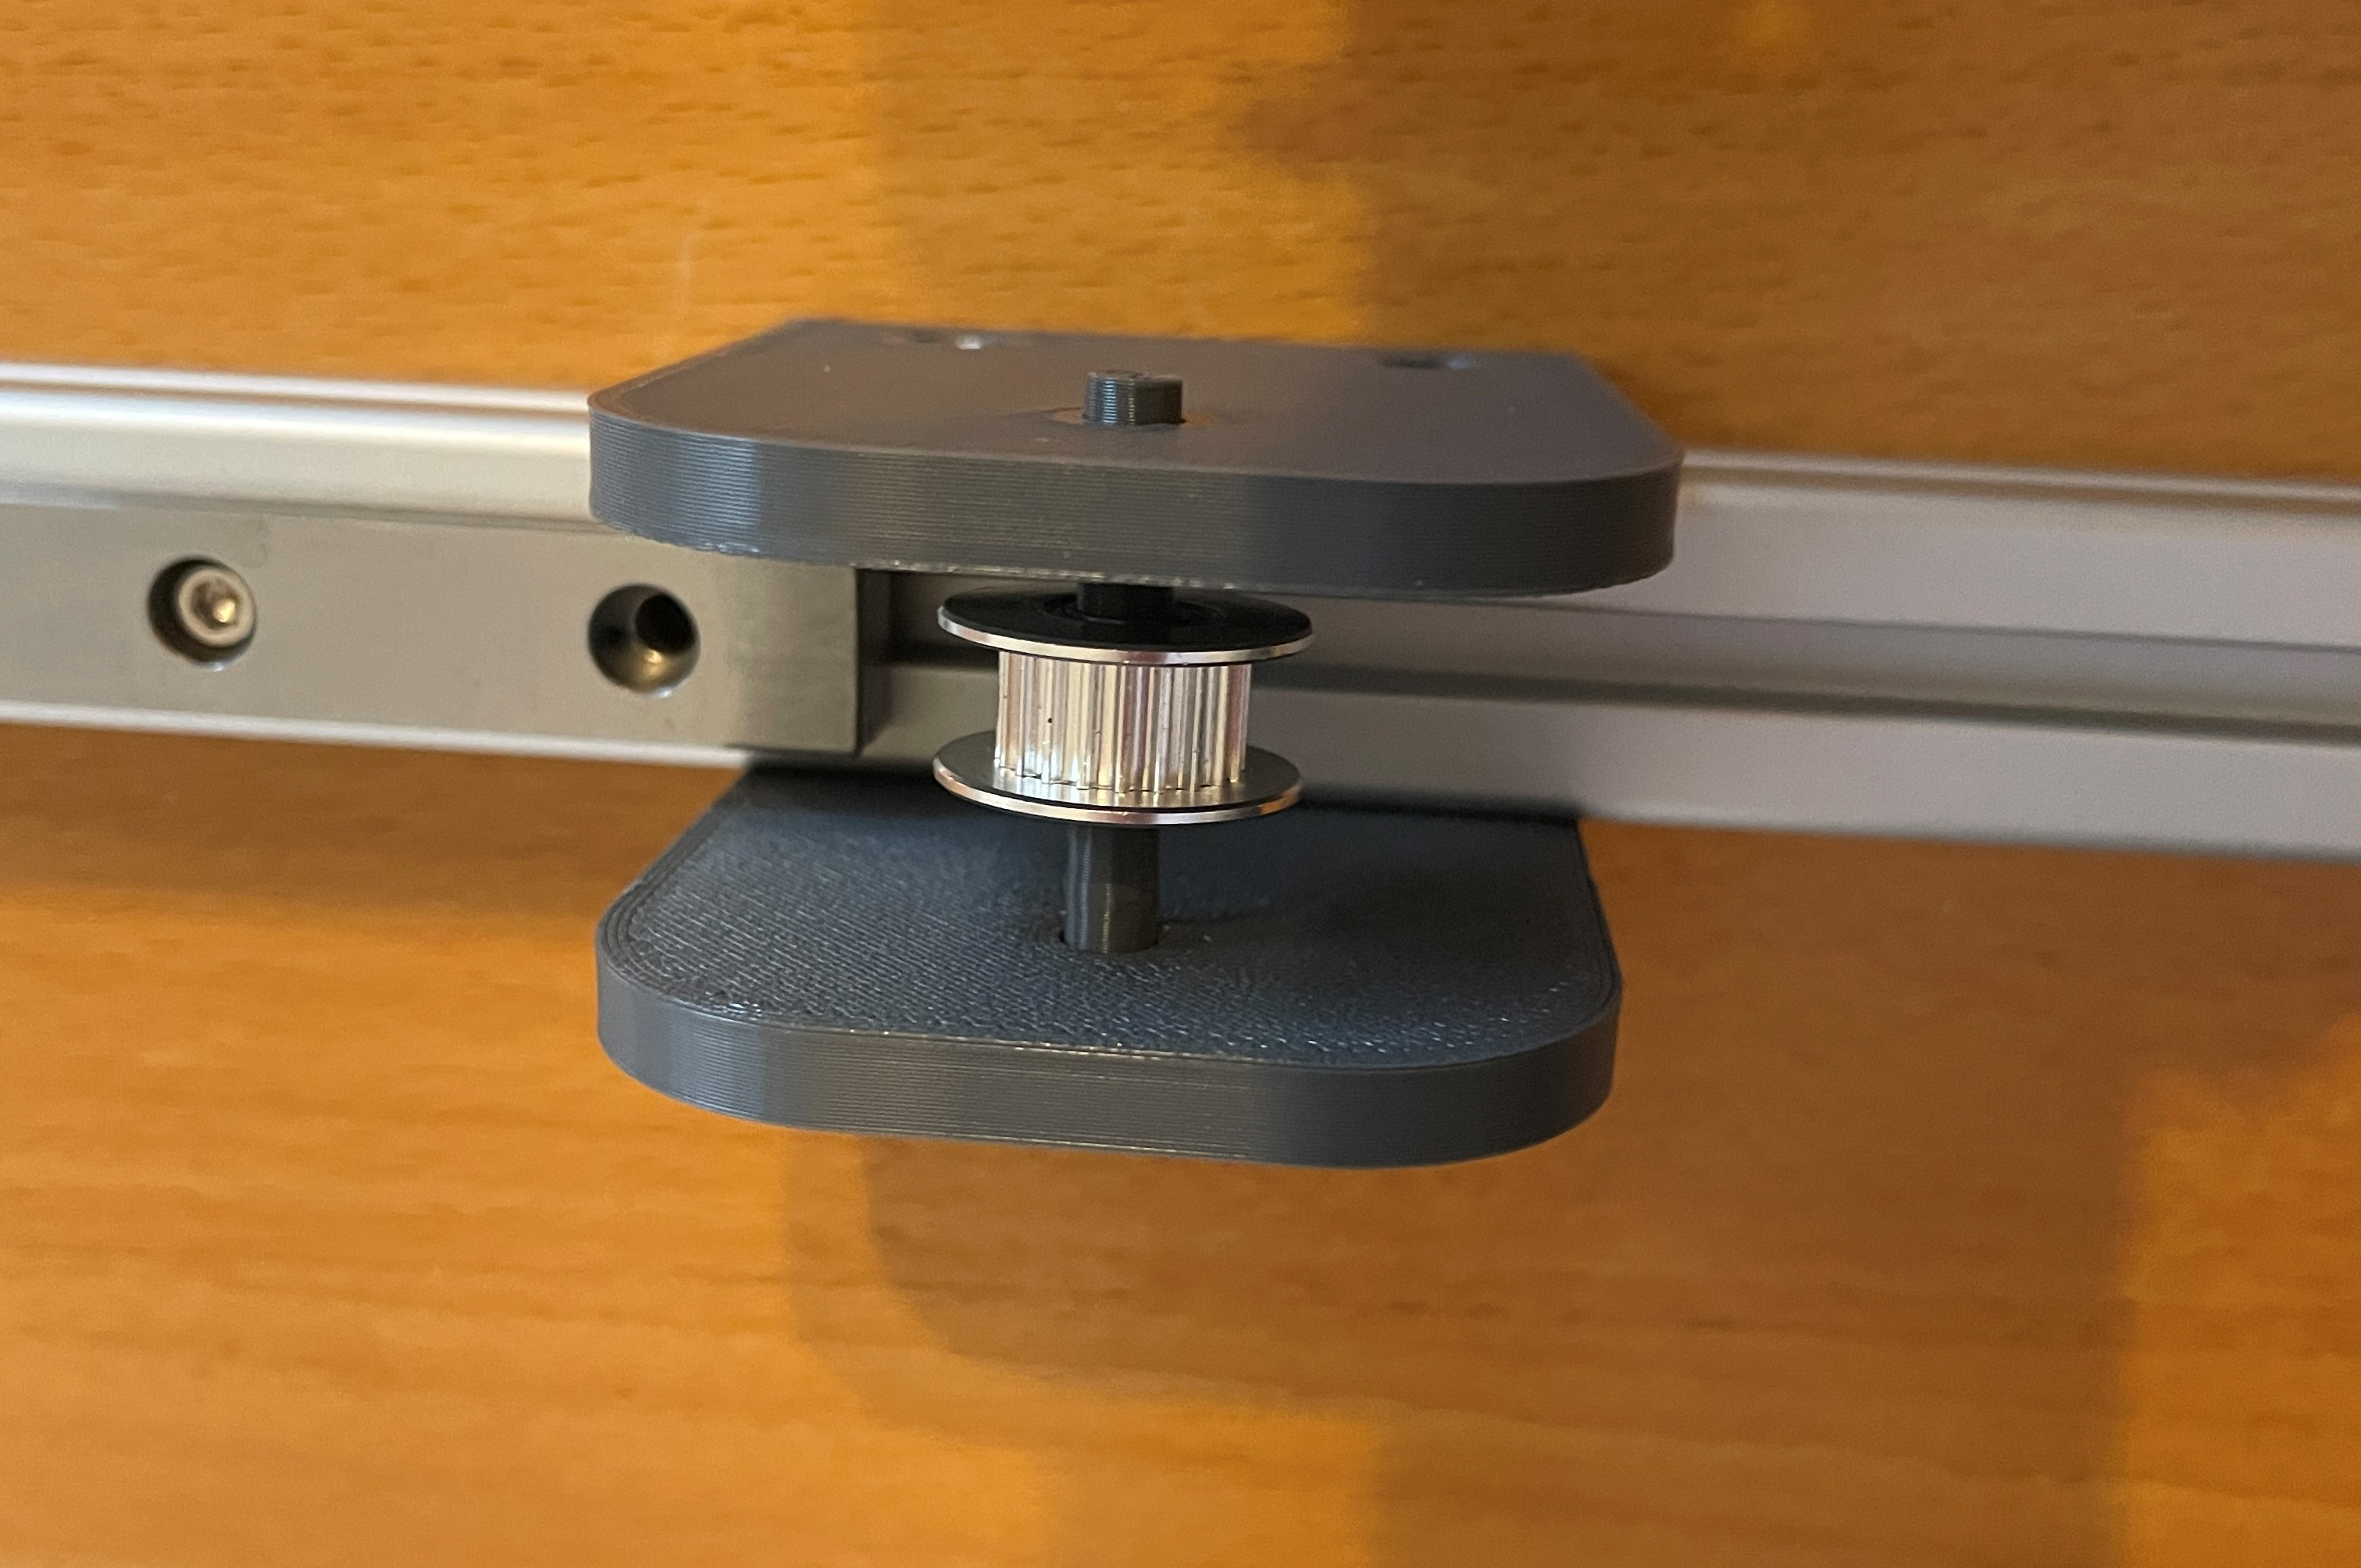
\includegraphics[width=\textwidth]{Images/11Schr.jpg}
		\caption{Elfter Schritt: Montieren der Halter für die Welle} \label{11.S}
	\end{center}
\end{figure}


\section{Zwölfter Schritt: Montieren der Riemenscheibe am Motor}

Montieren Sie die folgenden Bauteile wie in Abbildung \ref{11.S} gezeigt.

\begin{enumerate}
	\item Montieren Sie die Riemenscheibe auf die Welle des Nema 17 Motors und befestigen Sie den mit den Madenschrauben in der Riemenscheibe. 
\end{enumerate}

\begin{figure}[H]
	\begin{center}
		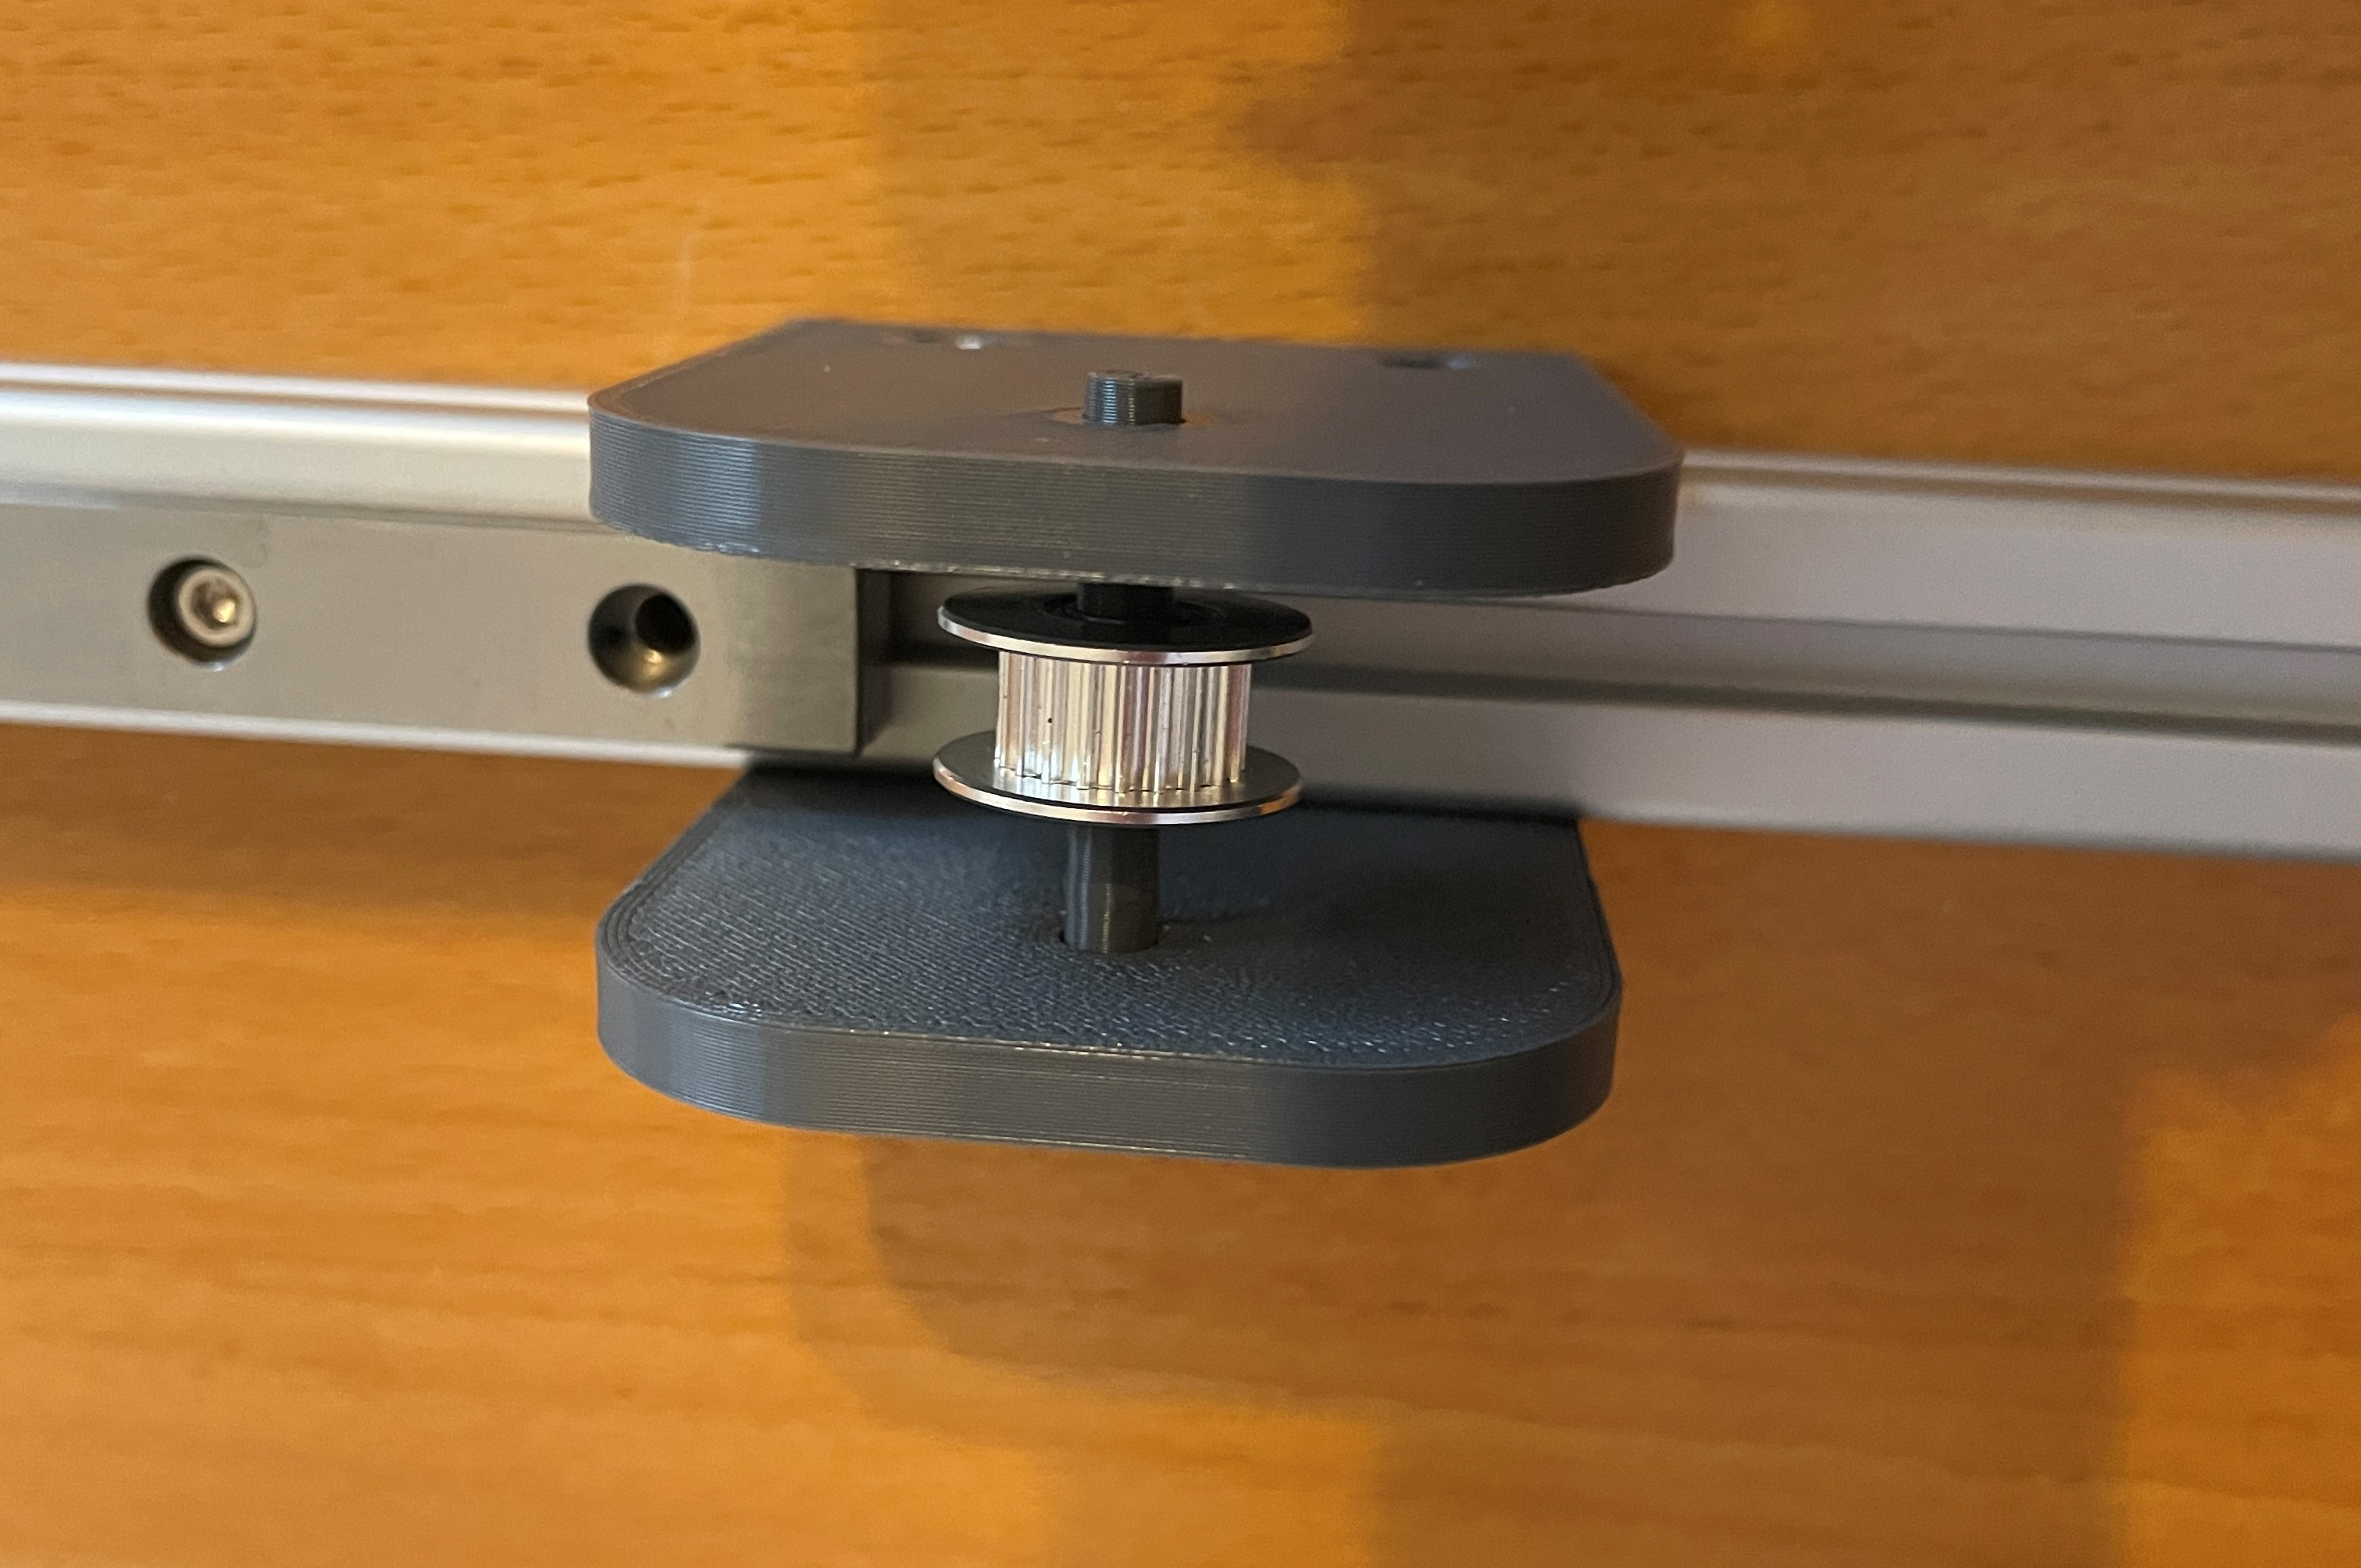
\includegraphics[width=\textwidth]{Images/11Schr.jpg}
		\caption{Zwölfter Schritt: Montieren der Riemenscheibe am Motor} \label{12.S}
	\end{center}
\end{figure}


\section{Dreizehnter Schritt: Montieren des Anzeigers und des Riemens}

Montieren Sie die folgenden Bauteile wie in Abbildung \ref{13.S} gezeigt.

\begin{enumerate}
	\item Montieren Sie den Anzeiger auf den Schlitten der Liniearführung mit 4 $\times$ $ M3 \times 6 \ mm $ Schrauben.
	\item Montieren Sie den Riemen Auf den Anzeiger mit 4 $\times$ $ M3 \times 6 \ mm $ Schrauben.
\end{enumerate}

\begin{figure}[H]
	\begin{center}
		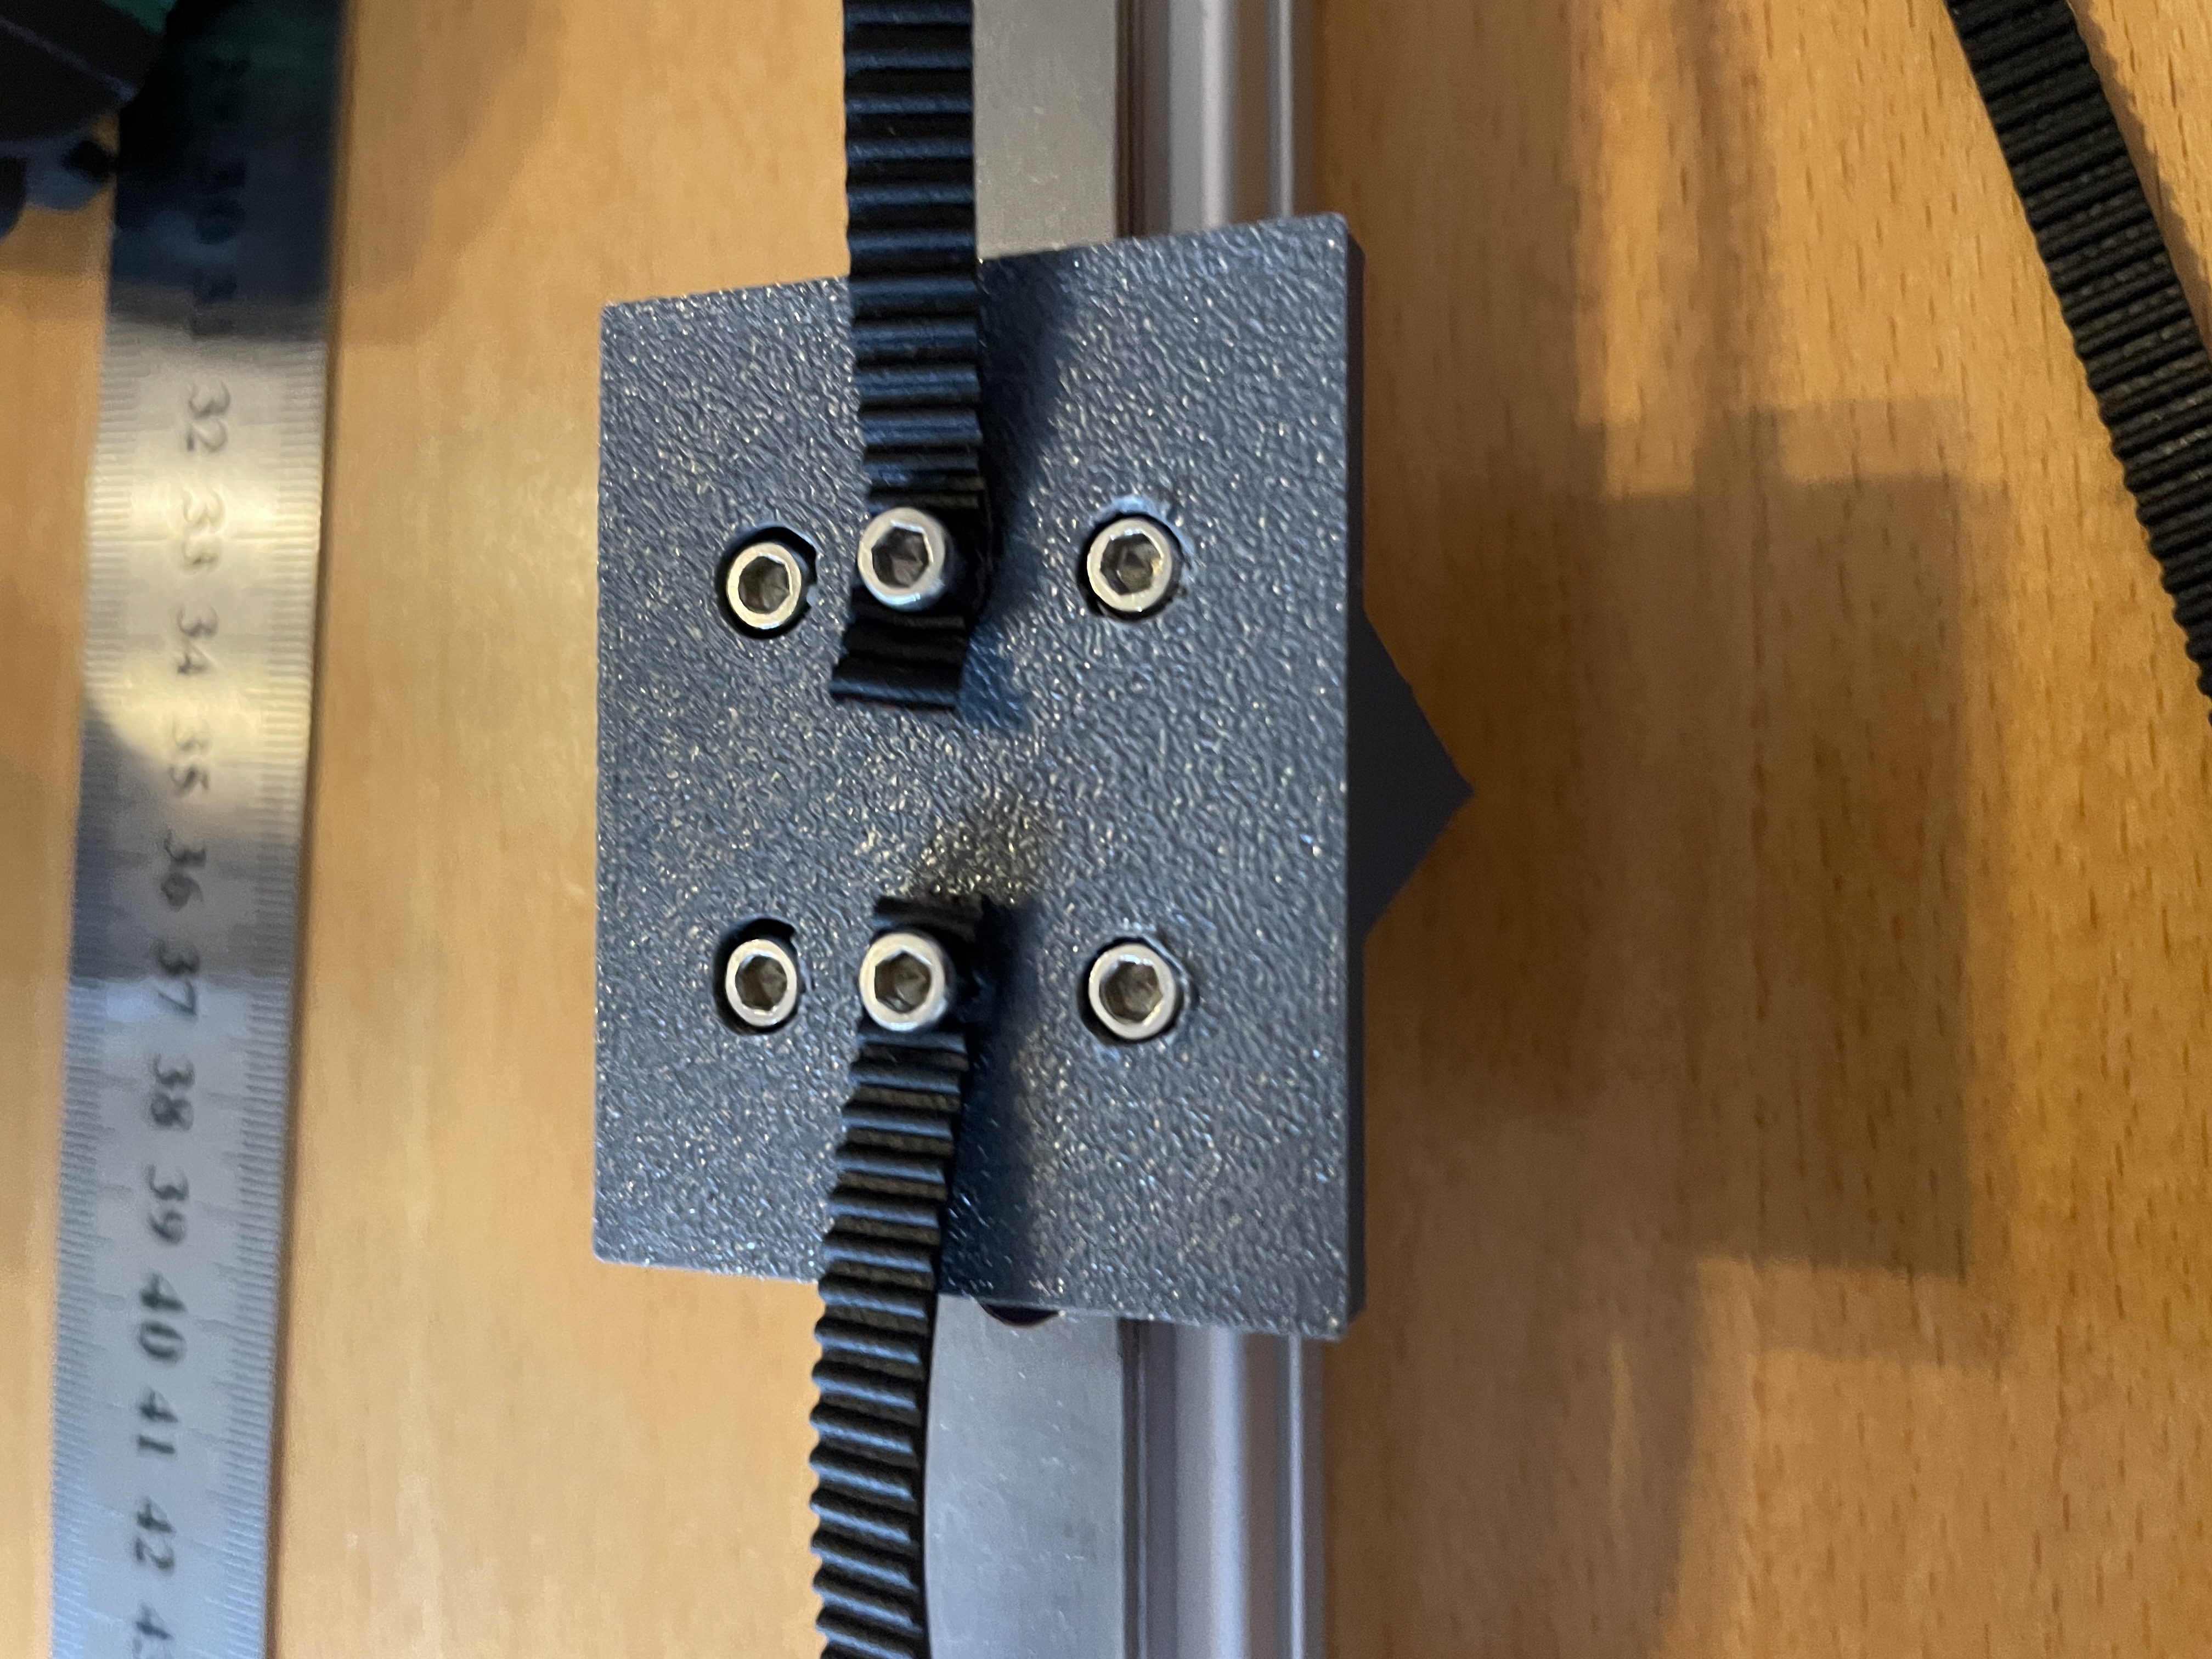
\includegraphics[width=\textwidth]{Images/13Schr.jpg}
		\caption{Zwölfter Schritt: Montieren des Anzeigers und des Riemens} \label{13.S}
	\end{center}
\end{figure}


\section{Vierzehnter Schritt: Montieren des Lineals}

\begin{enumerate}
	\item Montieren Sie das Lineal auf den Schlitten der Liniearführung mit 4 $\times$ $ M3 \times 6 \ mm $ Schrauben mit dem im Schritt 11 eingesetzten 2 $\times$ $ M3 $ Hammermutter.
\end{enumerate}


\section{Abschlussarbeiten}

\begin{enumerate}
	\item Überprüfen Sie alle Verbindungen und Schrauben auf festen Sitz.
	\item Testen Sie Mithilfe des Manuals die Funktionsfähigkeit des Demonstrators. 
\end{enumerate}
